% !TEX TS-program = xelatex
\documentclass[12pt]{article}
\usepackage{amsthm,amsmath,amssymb,braket,graphicx,enumitem,booktabs,multirow,booktabs,wrapfig,cancel,caption,fancyhdr,relsize,textpos,booktabs,tocbibind,titlesec,color}
\usepackage[margin=0.5in,bottom=0.6in]{geometry}
\graphicspath{{./figures/}}
\usepackage[T1]{fontenc}
\usepackage[pdfusetitle]{hyperref}
\renewcommand{\arraystretch}{2}
\setlength\delimitershortfall{-2pt}
\setcounter{tocdepth}{1}
\DeclareMathOperator{\sech}{sech}
\raggedbottom
\numberwithin{equation}{section}
\allowdisplaybreaks

\title{Generating Hubbard Model Solutions from Anderson Impurity Model Solutions}
\author{Abhirup Mukherjee, Dr. Siddhartha Lal}
\begin{document}
\maketitle
\tableofcontents
\newpage
\section{Introduction}
This is an attempt to obtain various quantities like Greens functions, self-energies, spectral functions and (if possible) energies and wavefunctions of the Hubbard model, using a cluster-bath approach. The cluster-bath system is taken to be a single-impurity Anderson model with a correlated bath. The correlation will be brought about in two ways: a self-energy $\Sigma(k,\omega)$ of the bath, and a double occupancy repulsion cost $U_b$. The Hubbard and the correlated single-impurity Anderson models are defined using the Hamiltonians
\begin{align}
H_\text{hubb} &= -t^H\sum_{\sigma,\left<i,j \right>}\left(c^\dagger_{i\sigma} c_{j\sigma} + \text{h.c.}\right) + U^H\sum_i \hat n_{i \uparrow} \hat n_{i \downarrow} - \mu^H \sum_{i\sigma}\hat n_{i\sigma}\\
H_\text{siam} &= \sum_{k\sigma}\left[\epsilon_k + \Sigma(k,\omega)\right]\hat n_{k\sigma} + \epsilon_d^A \sum_\sigma\hat n_{d\sigma} + U^A \hat n_{d \uparrow} \hat n_{d \downarrow} + U_b \sum_{kk^\prime}\hat n_k \hat n_{k^\prime} -t^A\sum_{k\sigma}\left(c^\dagger_{d\sigma}c_{k\sigma} + \text{h.c.}\right) \label{clus_bath_siam}
\end{align}
Broadly speaking, the method involves first solving the SIAM using a unitary renormalisation group approach, to get the low energy effective theory, and then combining the low energy Hamiltonians in a symmetrized fashion to get the Hamiltonian for the Hubbard model lattice. It is reminescent of dynamical mean-field theory (DMFT) - both involve an impurity-solver that solves an auxiliary system. The difference, however, lies in the following points:
\begin{itemize}
	\item While DMFT primarily works with Greens functions and self-energies, this method involves Hamiltonians. The impurity-solver in DMFT provides an impurity Greens function (which is then equated with the local Greens function of the bath), while the impurity-solver in this method actually provides a low energy Hamiltonian.
	\item The final step of DMFT is the self-consistency equation, where the impurity and bath-local quantities are set equal. This ensures all sites, along with the impurity site, have the same self-energy, something which is required on grounds of  translational invariance. The present method, however, brings about the translational invariance in a different way. It symmetrizes the Hamiltonians itself, such that all quantites then derived from the Hamiltonian are then guaranteed to have the symmetry.
\end{itemize}
The meaning of each of these statements will become clearer when we describe the method in more detail.

\section{Philosophy of the method}
The method is closely tied to the auxiliary system approach described in \cite{martin_2016}. We can view the full Hamiltonian as a sum of two component Hamiltonians \(H_1, H_2\) connected via the interaction term \(H_{12}\).
\begin{equation}\begin{aligned}
	H = \begin{pmatrix} H_1 && H_{12} \\ H_{12}^* && H_2 \end{pmatrix} = H_1 \ket{1}\bra{1} + H_2\ket{2}\bra{2} + H_{12}\ket{1}\bra{2} + H_{12}^*\ket{2}\bra{1}
\end{aligned}\end{equation}
where \(\ket{1(2)}\) actually represents a sum over all basis kets of the subsystem 1(2). As an example, we can split the the Hubbard model Hamiltonian between a particular site \(i = p\) and the rest of the lattice as follows:
\begin{equation}\begin{aligned}
	H_\text{hubb} &= \overbrace{U^H\hat n_{p \uparrow} \hat n_{p \downarrow} - \mu^H \sum_\sigma \hat n_{p \sigma}}^{H_1} \\
		      &+ \underbrace{U^H\sum_{i \neq p}\hat n_{i \uparrow} \hat n_{p \downarrow} - \mu^H \sum_{i \neq p, \sigma} \hat n_{i \sigma} -t^H\sum_{\sigma,\left<i,j \right>\atop{i \neq p \neq j}}\left(c^\dagger_{i\sigma} c_{j\sigma} + \text{h.c.}\right)}_{H_2}\\
		      & -\underbrace{t^H\sum_{\sigma,\atop{i \in \text{N.N. of }p}}\left(c^\dagger_{i\sigma} c_{p\sigma} + \text{h.c.}\right)}_{H_{12} + H_{12}^*}\\
\end{aligned}\end{equation}
The Greens function of the full Hamiltonian can also be split in a similar fashion:
\begin{equation}\begin{aligned}
	G(\omega) = \begin{pmatrix} G_1 && G_{12} \\ G_{12}^* && G_2 \end{pmatrix} 
\end{aligned}\end{equation}
The subsystem 1 is usually taken to be the "smaller system", and consequently, subsystem 2 represents the "bath".
The smaller system is typically chosen such that its eigenstates are known exactly.
Progress is then made by choosing a simpler version of the bath \(H_2\) and a simpler form also for its coupling \(H_{12}\) with the smaller system.
This combination of the smaller system and the simpler bath is then called the \textit{auxiliary system}.
A typical auxiliary system for the Hubbard model would be the SIAM, where the impurity represents an arbitrary site \(p\) of the lattice, the bath represents the rest of the lattice sites and the hybridisation term between the impurity and the bath represents the coupling term \(H_{12}\).
Such a construction is shown in fig.~\ref{cluster-bath}.
\begin{figure}[htpb!]
	\centering
	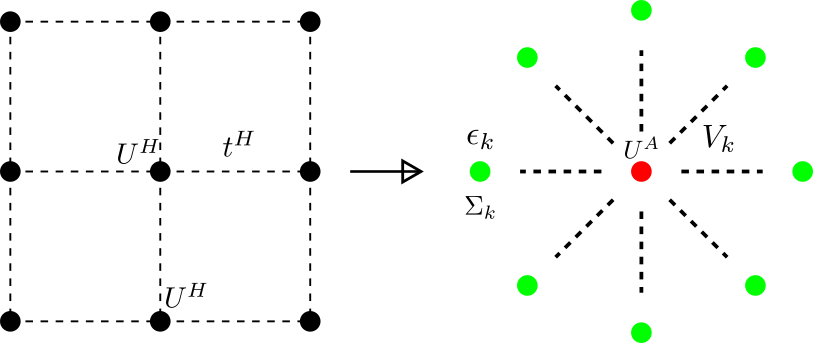
\includegraphics[width=0.8\textwidth]{cluster-bath.png}
	\caption{\textit{Left}: Full Hubbard model lattice with onsite repulsion $U^H$ on all sites and hopping between nearest neighbour sites with strength $t^H$. \textit{Right}: Extraction of the auxiliary (cluster+bath) system from the full lattice. The central site on left becomes the impurity site (red) on the right (with an onsite repulsion $\epsilon_d$), while the rest of the $N-1$ sites on the left form a conduction bath (green circles) (with dispersion $\epsilon_k$ and correlation modelled by the self-energy $\Sigma_k(\omega)$) that hybridizes with the impurity through the coupling $V$.}
	\label{cluster-bath}
\end{figure}
\textit{It should be noted that any reasonable choice of the cluster and bath would break the translational symmetry of the full model. To allow computing quantities, one would need to make the bath (which is a much larger system) simpler than the cluster (which is a single site). This distinction breaks the translational symmetry of the Hubbard model. For eg., if one chooses eq.~\ref{clus_bath_siam} as the auxiliary system, then the fact that the impurity has an onsite correlation while the bath only has a global capacitative cost $(\sim U_b N^2)$ means we have broken the symmetry between the cluster and the bath.}

The algorithm of DMFT then involves starting with some local self-energy of the bath, \(\Sigma(\omega)\), and using an impurity solver to calculate the impurity Greens function in the presence of this self-energy. This impurity Greens function is then used to calculate the impurity self-energy \(\Sigma_d(\omega)\), and the self-energy of the bath is then set equal to this impurity self-energy: \(\Sigma(\omega) = \Sigma_d(\omega)\), because we expect, on grounds of the lattice symmetry, that the impurity is the same as any other site in the bath. This is said to be the self-consistency step, because the bath self-energy is completely determined only at the end. With this updated bath self-energy, one then repeats the entire process until there is no further change in the bath self-energy at the self-consistency step.


The present method intends to calculate the quantities in a different fashion.
We start with a SIAM (with a correlated bath having a non-trivial self-energy), and solve it using the unitary renormalisation group approach to get to a fixed-point Hamiltonian.
The fixed point Hamiltonian will in general involve the impurity site (with renormalised parameters $\epsilon_d^*, U^*$) interacting with a smaller number of momentum states.
% Assuming the impurity-bath couplings are much larger than the dispersion of the bath, we can approximate the conduction bath part by a zero-mode of the kinetic energy part. The zero mode is defined as $c_0 = \frac{1}{\sqrt N}\sum_k c_k$, so it is just the zeroth site. 
% What this means is that all the momentum states will then collapse to a single site (which we call the zero mode site, and represents the origin of the lattice). We will also pick out the zeroth site part of the onsite correlation part, and replace that with a single correlation coupling $U^A_z$.
% Such a model, shown in fig.~\ref{and_mol} is exactly solvable.
At this point, we will assume that we have a Hubbard model in mind that has motivated a correlated SIAM as the auxiliary system, and we have performed renormalisation group analysis on this auxiliary system to get down to an effective Hamiltonian. We will also assume that the parameters of the auxiliary system have been chosen such that in the effective Hamiltonian, the impurity and zero mode have the same onsite repulsion: $U^A = U^A_z$ (this is required for translational invariance).
\\\\
To obtain a comparatively simple but physically well-motivated auxiliary model, we identify $\sum_k c_k = \sqrt N c_0$; \(c_0\) is the operator for the zeroth site (the site nearest to the impurity). We will call the set of all \(N-2\) sites apart from the impurity and this zeroth site as the "effective bath". The fixed point Hamiltonian can be separated into these parts: an isolated impurity part, an isolated zeroth site part, an isolated effective bath part, hopping between impurity and the zeroth site and hopping between the zeroth site and the effective bath. \textit{As a simplification, we will ignore the correlation term \((U)\) on the effective bath}. In preparation of a symmetrization procedure, we will relabel the impurity site as 0, and the zeroth site as 1. With all these steps, the Hamiltonian takes the form:
\begin{equation}\begin{aligned}
	% H^A_\text{corr} = -t^A\sum_{\sigma}\left(c^\dagger_{d\sigma}c_{z\sigma} + \text{h.c.}\right) + U^A\tau_{d \uparrow}\tau_{d \downarrow} + U^A_z\tau_{z \uparrow}\tau_{z \downarrow}
	\underbrace{U^A\tau_{0 \uparrow}\tau_{0 \downarrow} + U^A\tau_{1 \uparrow}\tau_{1 \downarrow}}_\text{imp. \& zero-mode isolated} - \underbrace{t^A\sum_{\sigma}\left(c^\dagger_{0\sigma}c_{1\sigma} + \text{h.c.}\right)}_\text{0-1 coupling} - \underbrace{t^A\sum_{j \in \atop{\text{NN of 1}}}\left(c^\dagger_{1\sigma}c_{j\sigma} + \text{h.c.}\right)}_\text{1 \& eff. bath coupling} - \underbrace{t^A \sum_{\left<ij \right>}^{\text{eff.} \atop{\text{bath}}}\left(c^\dagger_{i\sigma}c_{j\sigma} + \text{h.c.}\right)}_\text{eff. bath isolated}
\end{aligned}\end{equation}
\begin{figure}[htpb]
	\centering
	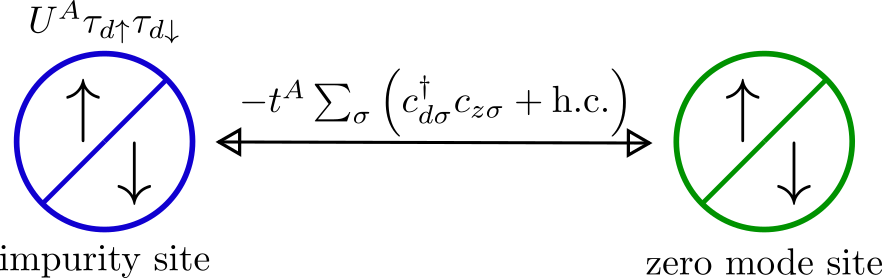
\includegraphics[width=0.6\textwidth]{gen_siam.png}
	\caption{Correlated asymmetric Anderson molecule schematic version. It consists of an impurity site (blue) hybridising with a bath (ring) by hopping into and out of the zeroth site (pink). The other sites (green) form the rest of the bath. Just the impurity site and the zeroth site have onsite repulsion.}
	\label{and_mol}
\end{figure}
This Hamiltonian is depicted in fig.~\ref{and_mol}. Such a Hamiltonian is, however, explicitly asymmetric between the sites 0 and 1 (the effective bath couples only to 1). To rectify that, we will symmetrize the coupling between the effective bath and the sites 0 and 1, by exchanging the sites 0 and 1. The resultant Hamiltonian is
\begin{equation}\begin{aligned}
	\underbrace{U^A\tau_{0 \uparrow}\tau_{0 \downarrow} + U^A\tau_{1 \uparrow}\tau_{1 \downarrow} - t^A\sum_{\sigma}\left(c^\dagger_{0\sigma}c_{1\sigma} + \text{h.c.}\right)}_\text{2-site Hubbard model} +\underbrace{- t^A\sum_{j \in \atop{\text{NN of 1}}}\left(c^\dagger_{1\sigma}c_{j\sigma} + \text{h.c.}\right)- t^A\sum_{j \in \atop{\text{NN of 0}}}\left(c^\dagger_{0\sigma}c_{j\sigma} + \text{h.c.}\right)}_\text{dimer \& eff. bath coupling} \\
	- \underbrace{t^A \sum_{\left<ij \right>}^{\text{eff.} \atop{\text{bath}}}\left(c^\dagger_{i\sigma}c_{j\sigma} + \text{h.c.}\right)}_\text{eff. bath isolated}
\end{aligned}\end{equation}
% The motivation for extracting the zero mode is that it leads to a very simple effective Hamiltonian (the asymmetric Anderson molecule) without losing much of the low energy physics.
To further simplify this Hamiltonian, \textit{we will combine the nearest neighbour sites of \(1\) and \(0\) into a single site}.
\begin{equation}\begin{aligned}
	c_z \equiv \left(\sum_{j \in \atop{\text{NN of 1}}} + \sum_{j \in \atop{\text{NN of 0}}}\right)c_{j}
\end{aligned}\end{equation}
This single site will act as the zeroth site of the effective bath, and it means that both sites of the Hubbard dimer hybridizes with the effective through just a single site. With this assumption, the Hamiltonian for "a Hubbard dimer hopping into an effective bath" takes the simple form
\begin{equation}\begin{aligned}
	\label{dimer_p_bat}
	\tilde H^D = H^D(0,1) - t^D \sum_{\sigma}\left(c^\dagger_{0\sigma}c_{z\sigma} + c^\dagger_{1\sigma}c_{z\sigma} + \text{h.c.}\right) + \sum_{\vec k}^\text{eff. bath}\epsilon_{\vec k}\hat n_{\vec k}
\end{aligned}\end{equation}
\(H^D(0,1)\) is the Hubbard dimer Hamiltonian (shown in fig.~\ref{hubb-dim}):
\begin{equation}\begin{aligned}
	\label{dimer_ham}
	H^D(0,1) \equiv -t^D\sum_\sigma\left( c^\dagger_{0\sigma}c_{1\sigma} + \text{h.c.} \right) + U^D\left( \tau_{0 \uparrow}\tau_{0 \downarrow} + \tau_{1 \uparrow}\tau_{1 \downarrow}\right)
\end{aligned}\end{equation}
\begin{figure}[htpb!]
	\centering
	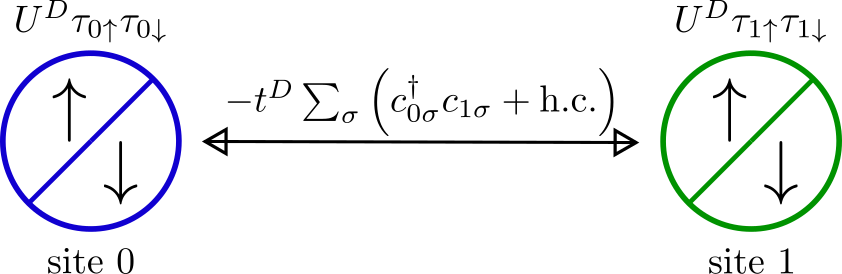
\includegraphics[width=0.4\textwidth]{hubb_dim.png}
	\caption{Hubbard dimer schematic version. It again consists of two sites, like the Anderson molecule, but now both sites have onsite repulsion, and their is again inter-site hopping.}
	\label{hubb-dim}
\end{figure}
This entire procedure is depicted in fig.~\ref{dimer-bath}.
\begin{figure}[htpb]
	\centering
	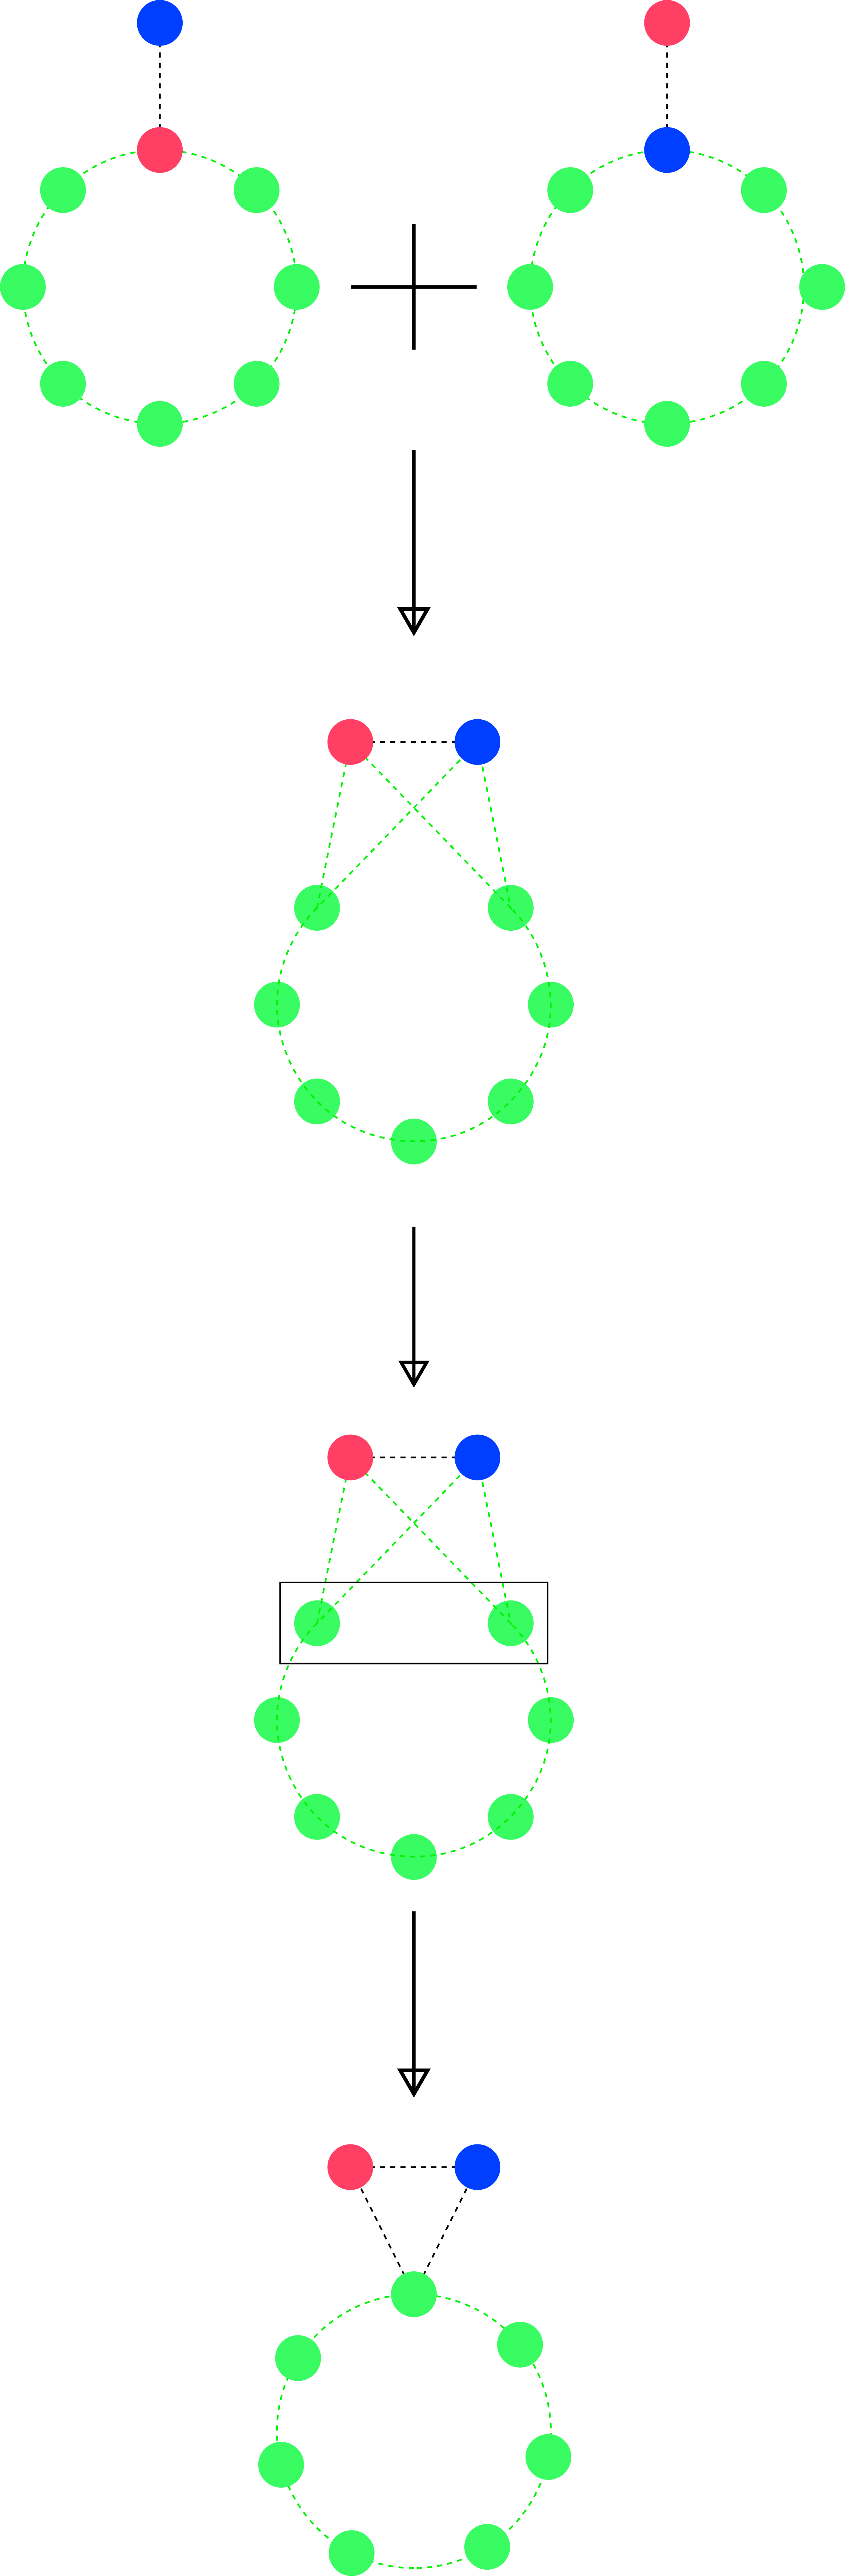
\includegraphics[width=0.3\textwidth]{dimer_bath.png}
	\caption{The process of symmetrizing the Rg fixed point Hamiltonian and then creating a dimer+bath Hamiltonian. We first add the asymmetric Hamiltonians to get a symmetrized Hamiltonian. In the symmetrized Hamiltonian, the dimer has \(w\) entry points into the bath, \(w\) being the coordination number of the lattice. We then merge these \(w\) lattice sites (enclosed in the black box) into a single lattice site.}
	\label{dimer-bath} 
\end{figure}
We  can thus obtain a family of Hamiltonians \(\tilde H^D(i,j)\) obtained by setting \(0\) and \(1\) by setting the two sites of the dimer to any nearest-neighbour \(i,j\) on the lattice and the effective bath to the rest \(N-2\) sites of the lattice. The next step in the programme is to tile the real-space lattice with this dimer+bath Hamiltonian \(\tilde H_D\) to restore translational invariance (shown in a later section), and obtain a new Hubbard Hamiltonian, $\tilde H = T\left[ \tilde H^{D} \right] T^{-1}$, where $T$ denotes the operator that performs the set of iterative real-space translations, and enables the dimer Hamiltonian to span the target real-space lattice. We quote the final form of $\tilde H$ here to explain what the tiling means, but the explanation is given in a later section.
\begin{equation}\begin{aligned}
	\tilde H &= \frac{2}{Nw}\sum_{\left<ij\right>}\frac{1}{2(w-1)}\sum_{l \in \text{NN of (i,j)}}\tilde H^D((0,1,z) \to (i, j, l))\\
		 &= \frac{2}{N}U^D\sum_{i} \tau_{i \uparrow}\tau_{i \downarrow} - \frac{2}{Nw}\left(1 + \frac{Nw}{2}\right)t^D\sum_{\left<ij\right>}\left(c^\dagger_{i\sigma}c_{j\sigma} + \text{h.c.}\right)
\end{aligned}\end{equation}
What that means is that we have placed the Hubbard dimer+bath system at all nearest neighbour pairs to reconstruct a new Hubbard model. If we assume that the tiling mostly rectifies the explicit symmetry-breaking made while choosing the auxiliary system as well as dropping the correlation on the bath sites, we can write
\begin{equation}\begin{aligned}
	\label{app2}
	\tilde H = \mathcal{U} H^H \mathcal{U}^{-1} = TZ\left[\mathcal{U}_A H^A \mathcal{U}_A^\dagger \right]Z^{-1} T^{-1}~,
\end{aligned}\end{equation}
where $\mathcal{U} = TZ\mathcal{U}_{A}$ is some transformation that is either a unitary, or, at the very least, a similarity transformation that maps from the original to the reconstructed Hubbard Hamiltonian. 
The existence of $U$ is contingent on how good the approximations are.
\\\\
We mention the two approximations made along the entire journey from the original Hubbard model to the reconstructed one here.
\begin{itemize}
	\item We have replaced the full Hubbard model by an auxiliary system described by the SIAM Hamiltonian in eq.~\ref{clus_bath_siam}. The accuracy of this assumption is determined by the choice of the SIAM parameters, particular the self-energy and repulsion of the bath. As discussed before, the very choice of th cluster and bath spoil the translational invariance of the parent model.
	\item We then perform a unitary RG on $H^A$. This leads to a fixed-point Hamiltonian $\mathcal{U}_A H^A \mathcal{U}_A^\dagger$. At this point, we go from the fixed point Hamiltonian to the dimer+bath Hamiltonian in eq.~\ref{dimer_p_bat}. If we represent this transformation from the fixed point Hamiltonian to the Hamiltonian in eq.~\ref{dimer_p_bat} by an operator \(Z\), we can write $H^D = Z\left[\mathcal{U}_A H^A \mathcal{U}_A^\dagger \right] Z^{-1}$. This constitutes the second approximation we make.
\end{itemize}

\section{Spectral function of the single-impurity Anderson model}
To get a better look at what we are getting into and what we should expect going forward, we first calculate the spectral function of the smaller single-impurity Anderson model that is obtained as the low-energy Hamiltonian of an URG analysis of the full SIAM. This ow energy effective Hamiltonian is
\begin{equation}\begin{aligned}
	\epsilon_d \hat n_d + U\hat n_{d \uparrow} \hat n_{d \downarrow} + v \left(c^\dagger_{d\sigma}c_{0\sigma} + \text{h.c.}\right) + \sum_{k \in \left[-\Lambda^*, \Lambda^*\right], \sigma}\epsilon_k \hat n_{k\sigma}
\end{aligned}\end{equation}
All the impurity couplings are fixed point values, and the momentum states of the bath now run over a reduced bandwidth. The subscript \(d\) indicates that the operator is that of the impurity, while the subscript \(0\) indicates it is of the zeroth site of the bath: \(c_0 = \frac{1}{\sqrt N}\sum_k c_k\). The spectral function of the SIAM is already known from other methods like the numerical renormalization group. For small values of \(U\), the spectral function consists of just the central quasiparticle excitation peak. At larger values of \(U\), we see the emergence of the two Hubbard side bands while the spectral weight at the centre decreases. We also calculated the spectral function of the low energy theory sing exact diagonalization. The plots are shown in fig.~\ref{siam_spec_func}.
\begin{figure}[htpb]
	\centering
	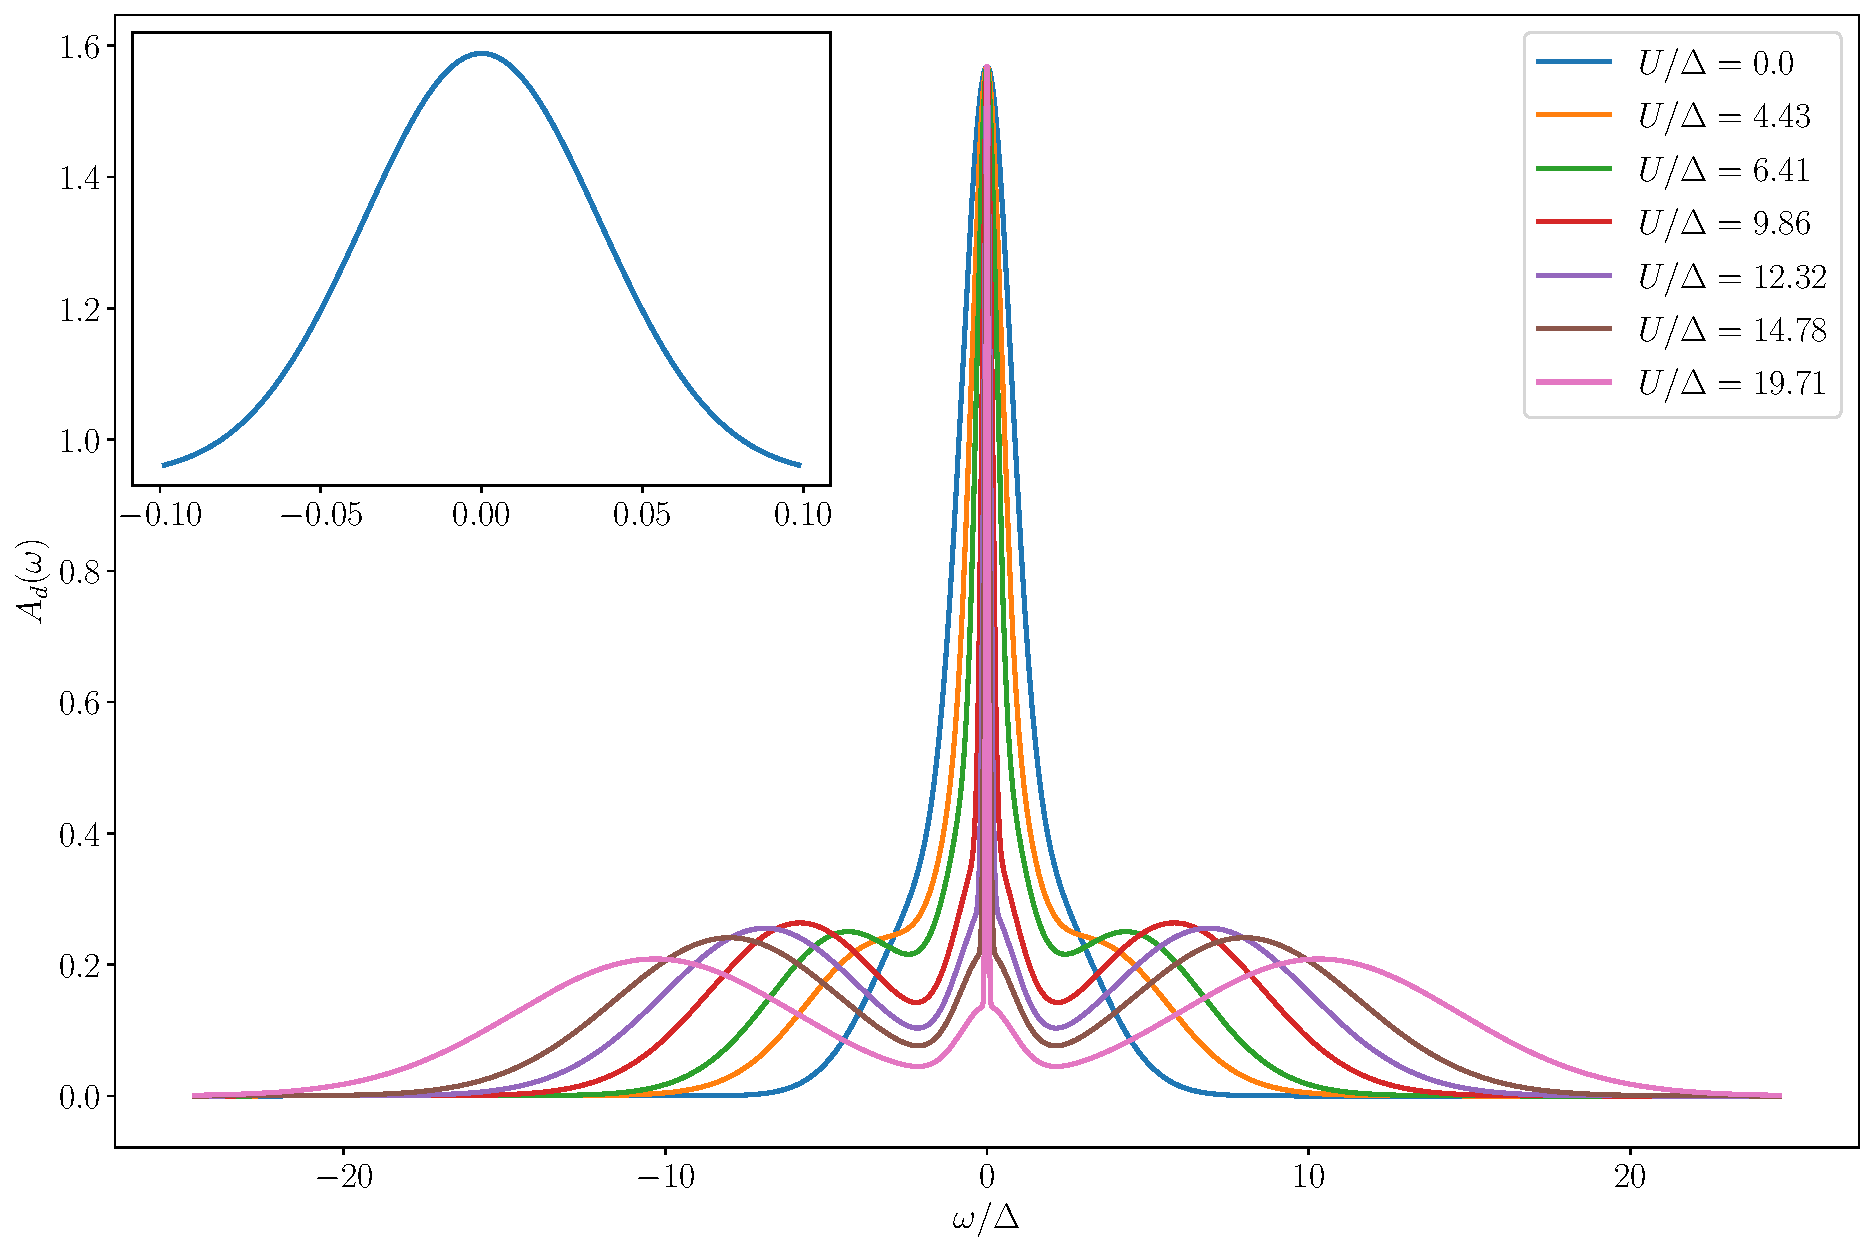
\includegraphics[width=0.9\textwidth]{./siam_specfunc_all.pdf}
	\caption{Spectral function of the effective SIAM Hamiltonian for various values of \(\frac{U}{\Delta}\). \(\Delta\) is defined by the height of the central peak in the non-interacting model \(U=0\). The inset shows a zoom-in of the final spectral function \(\left( \frac{U}{\Delta} = 19.71 \right)\) near \(\omega = 0\).}
	\label{siam_spec_func}
\end{figure}
\\\\
Because we kept only a discrete bath of 4 momentum states, \textit{we had to artificially enforce the constancy of the height of the central peak.} To convert the delta functions into a continuous spectrum, we  The central peak (or equivalently, the central pole in the impurity Greens function) does not vanish even for exhorbitantly large values of \(\frac{U}{\Delta}\), implying that there is no stable local moment phase in the SIAM (a local moment phase would involve a gap at zero frequency in the impurity spectral function). Formally, the local moment phase will be stable only at \(U \to \infty\) or \(v^* = 0\).
\\\\
We also checked how the width of the central peak varies with increasing \(U\). The behaviour is shown in fig.~\ref{fwhm}. The width was also fitted against a function, as shown in the plot.
\begin{figure}[htpb]
	\centering
	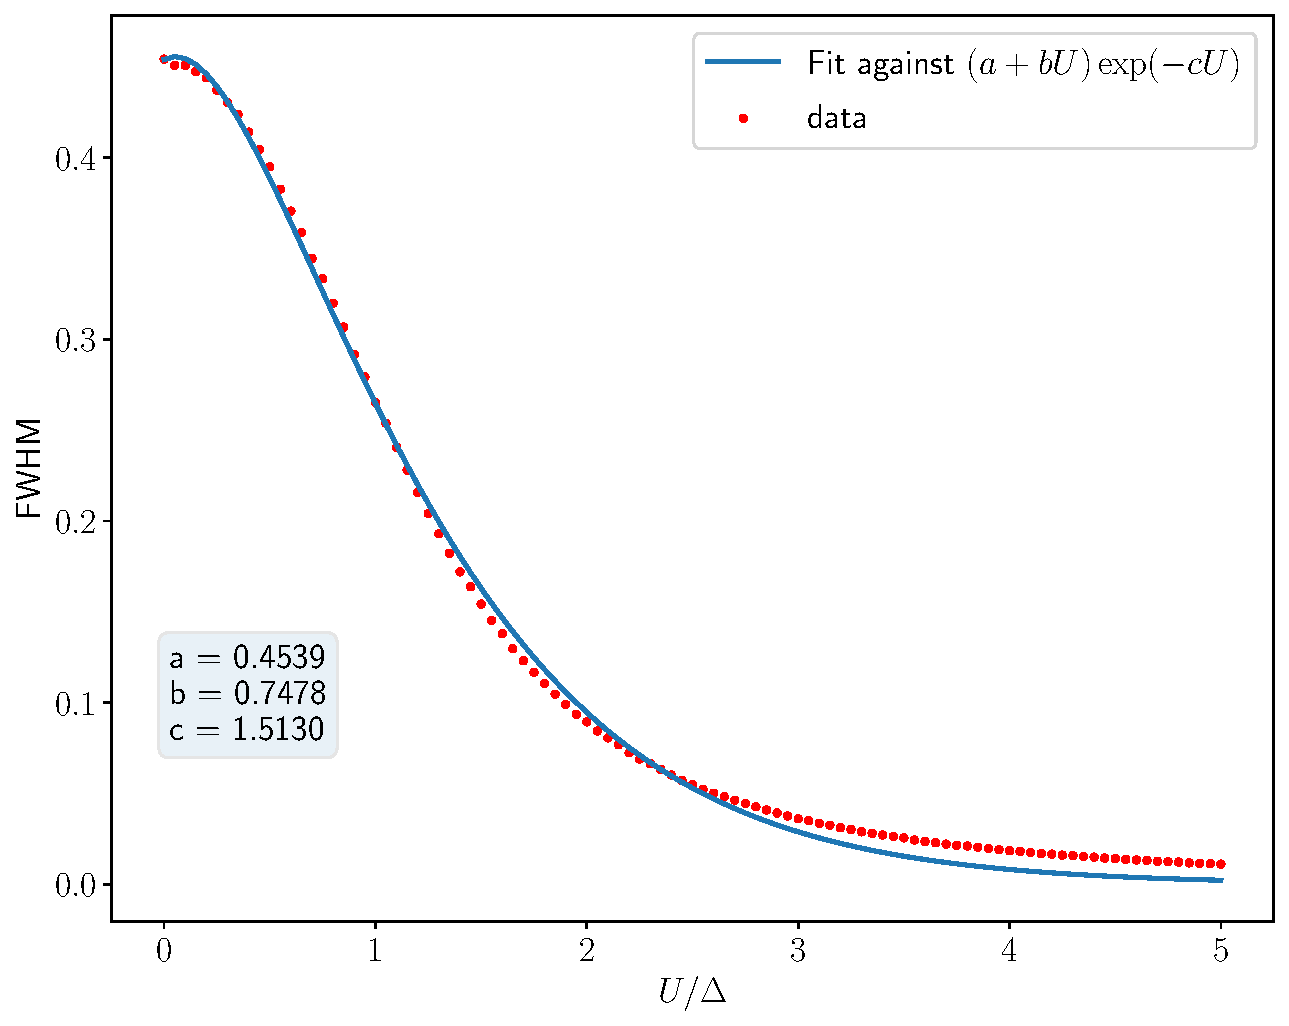
\includegraphics[width=0.6\textwidth]{./width_vs_U_simple_fit.pdf}
	\caption{The decay of the full width at half maximum (FWHM) of the central peak, with increasing \(\frac{U}{\Delta}\). The behaviour satisfies a function of the form shown in the legend.}
	\label{fwhm}
\end{figure}

\section{Spectral function of a correlated SIAM}
Since the SIAM cannot show a transition from a metallic (Fermi liquid) phase to a local moment phase, we next consider the slightly more correlated version where the zeroth site (which the impurity couples to) now has a Hubbard repulsion.
\begin{equation}\begin{aligned}
	\epsilon_d \hat n_d + U\hat n_{d \uparrow} \hat n_{d \downarrow} + U_b\hat n_{0 \uparrow} \hat n_{0 \downarrow} + v \left(c^\dagger_{d\sigma}c_{0\sigma} + \text{h.c.}\right) + \sum_{k \in \left[-\Lambda^*, \Lambda^*\right], \sigma}\epsilon_k \hat n_{k\sigma}
\end{aligned}\end{equation}
In such a model, if the impurity is to hybridize with the bath, it has to hop onto the zeroth site, but that site now has a double-occupancy cost. As a result, this new physics makes it harder for the impurity electron to delocalise, and suggests that there might be a metal-insulator transition at some critical value of the impurity \(U\), and this critical value should itself be a function of \(U_b\). This model therefore provides a tool for showing the changes in the phase diagram of the SIAM. Without any correlation in the bath, the SIAM has just one stable fixed point, the strong-coupling one. Starting up a correlation on the zero mode allows us to examine how this scenario might change if we have a correlated bath. One can also draw a comparison to DMFT and argue that such a model is similar to that stage of DMFT when the process has gone through a few steps of self-consistency enforcement and the bath itself has started to become correlated.
\\\\
Apart from its importance as a standalone problem, this correlated SIAM also sets the stage for a fully-symmetrized auxiliary model, the Hubbard dimer in a bath. In other words, by taking a symmetric combination of the correlated SIAM Hamiltonians (the symmetrization is done by exchanging the impurity and bath zero mode sites), one can obtain the Hamiltonian of a dimer hybridising with a bath, as shown in eq.~\ref{dimer_p_bat}. Such a symmetrised Hamiltonian should presumably correspond to a DMFT final-stage Hamiltonian, because the impurity and bath zero mode sites are now completely symmetric.

\section{Solution of the Hubbard dimer using the Anderson molecule}
This section tries to see how far we can we can go if we just work with the Anderson molecule as the smallest unit of tiling. We will attempt to reproduce the entire spectrum of a Hubbard dimer by creating a new Hamiltonian made up purely of Anderson molecules. This will guide us in deciding how to generalize the "tiling method" for a general $N-$site Hubbard model, as well as give indications as to whether we need a different smallest unit for tiling.
\\\\
The Hubbard dimer and Anderson molecules (zero-mode) are defined by the following respective Hamiltonians:
\begin{equation}\begin{aligned}
	H^H &= -t^H\sum_{\sigma}\left(c^\dagger_{1\sigma}c_{2\sigma} + \text{h.c.}\right) + U^H\sum_{i=1,2}\hat n_{i \uparrow}\hat n_{i \downarrow} - \mu^H \sum_{\sigma, i=1,2}\hat n_{i\sigma}\\
	H^A &= -t^A\sum_{\sigma}\left(c^\dagger_{d\sigma}c_{z\sigma} + \text{h.c.}\right) + \epsilon_d^A \sum_{\sigma}\hat n_{d\sigma} + U^A\hat n_{d \uparrow}\hat n_{d \downarrow}
\end{aligned}\end{equation}
In the first Hamiltonian, the indices \(i=1,2\) refer to the two lattice sites that constitute the dimer. In the second Hamiltonian, the subscript \(d\) indicates the impurity site, while the subscript \(z\) indicates the zero-mode site. First, we will assume that the Hubbard dimer is at half-filling (\(\frac{1}{2}U^H = \mu^H\)):
\begin{equation}\begin{aligned}
	\label{hubb_dimer}
	H^H &= -t^H\sum_{\sigma}\left(c^\dagger_{1\sigma}c_{2\sigma} + \text{h.c.}\right) + U^H\sum_{i=1,2}\hat \tau_{i \uparrow}\hat \tau_{i \downarrow} + \left(\frac{1}{2}U^H- \mu^H\right) \sum_{\sigma, i=1,2}\hat n_{i\sigma} + \text{constant}\\
	    &= -t^H\sum_{\sigma}\left(c^\dagger_{1\sigma}c_{2\sigma} + \text{h.c.}\right) + U^H\sum_{i=1,2}\hat \tau_{i \uparrow}\hat \tau_{i \downarrow}
\end{aligned}\end{equation}
Since the Hubbard Hamiltonian is at half-filling, we will also place the impurity at half-filling by setting \(\epsilon_d^A = -\frac{1}{2}U^A\):
\begin{equation}\begin{aligned}
	\label{and_dimer}
	H^A &= -t^A\sum_{\sigma}\left(c^\dagger_{d\sigma}c_{z\sigma} + \text{h.c.}\right) + \left(\epsilon_d^A + \frac{1}{2}U^A\right) \sum_{\sigma}\hat \tau_{d\sigma} + U^A\hat \tau_{d \uparrow}\hat \tau_{d \downarrow} + \text{constant}\\
	    &= -t^A\sum_{\sigma}\left(c^\dagger_{d\sigma}c_{z\sigma} + \text{h.c.}\right) + U^A\hat \tau_{d \uparrow}\hat \tau_{d \downarrow}
\end{aligned}\end{equation}
The first step is to recreate the Hubbard dimer Hamiltonian eq.~\ref{hubb_dimer} using the Anderson molecule Hamiltonian eq.~\ref{and_dimer}:
\begin{equation}\begin{aligned}
	H^H &= -t^H\sum_{\sigma}\left(c^\dagger_{1\sigma}c_{2\sigma} + \text{h.c.}\right) + U^H\sum_{i=1,2}\hat \tau_{i \uparrow}\hat \tau_{i \downarrow}\\
	    &= \frac{1}{2}\left[-t^H\sum_{\sigma}\left(c^\dagger_{1\sigma}c_{2\sigma} + \text{h.c.}\right) + t^H\sum_{\sigma}\left(c^\dagger_{2\sigma}c_{1\sigma} + \text{h.c.}\right)\right] + \frac{1}{2} 2U^H\sum_{i=1,2}\hat \tau_{i \uparrow}\hat \tau_{i \downarrow}\\
	    &= \frac{1}{2}\left[-t^A\sum_{\sigma}\left(c^\dagger_{d\sigma}c_{z\sigma} + \text{h.c.}\right)\bigg\vert_{z \to 2, d \to 1\atop{t^A \to t^H}} + t^A\sum_{\sigma}\left(c^\dagger_{2\sigma}c_{1\sigma} + \text{h.c.}\right)\bigg\vert_{d \to 2,z \to 1\atop{t^A \to t^H}} \right] \\
	    &+ \frac{1}{2} \left(U^A\hat \tau_{i \uparrow}\hat \tau_{i \downarrow}\bigg\vert_{d \to 1\atop{U^A \to 2U^H}} + U^A\hat \tau_{i \uparrow}\hat \tau_{i \downarrow}\bigg\vert_{d \to 2\atop{U^A \to 2U^H}}\right)\\
	    &=\frac{1}{2}\left[H^A\left(t^A \to t^H, U^A \to 2U^H, d \to 1, z \to 2\right) + H^A\left(t^A \to t^H, U^A \to 2U^H, d \to 2, z \to 1\right)\right]
\end{aligned}\end{equation}
The conclusion we can draw from this is that the Hubbard dimer Hamiltonian can be obtained from the Anderson dimer Hamiltonian in the following fashion:
\begin{itemize}
	\item The essential idea is that we have to create a local Hubbard Hamiltonian for each site of the Hubbard lattice by replacing the impurity label \(d\) in the Anderson dimer with the label of the particular site. So if there are two sites, we will get two local Hamiltonians obtained by replacing \(d\) with 1 and 2 respectively. For each local Hamiltonian, the zero-mode label \(z\) is replaced by the site that is nearest to the one that \(d\) is being replaced by. So, if \(d \to 1(2)\), then \(z \to 2(1)\).
	\item This, however, is not the only change that we must make, in order to get the local Hamiltonian for a particular site. Along with \(d\) and \(z\), we must also make the transformations \(t^A \to t^H, U^A \to 2U^H\).
	\item Finally, once we have the local Hamiltonians for sites 1 and 2, we average them to get the total Hubbard Hamiltonian.
\end{itemize}
Note that we expect most of these "rules" to be specific for the dimer, and there will be generalizations to most of them for a general \(N-\)site Hubbard Hamiltonian.


The wavefunctions for the \(N=2\) sector can also be connected through these transformations. Since both the Hamiltonians are analytically solvable, we can write down their groundstate wavefunctions \cite{pavarini}:
\begin{equation}\begin{aligned}
	\ket{\Psi^H_\text{GS}} &= a_1(U^H, t^H)\frac{1}{\sqrt 2}\left(\ket{\uparrow_1, \downarrow_2} - \ket{\downarrow_1, \uparrow_2}\right) - a_2(U^H,t^H){\sqrt 2}\left(\ket{\uparrow_1\downarrow_1, } - \ket{,\uparrow_2\downarrow_2}\right)\\
	\ket{\Psi^A_\text{GS}} &= a_1(\frac{1}{2}U^A, t^A)\frac{1}{\sqrt 2}\left(\ket{\uparrow_d, \downarrow_z} - \ket{\downarrow_d, \uparrow_z}\right) - a_2(\frac{1}{2}U^A,t^A){\sqrt 2}\left(\ket{\uparrow_d\downarrow_d, } - \ket{,\uparrow_z\downarrow_z}\right)\\
	E^H_\text{GS} &=  -\frac{1}{2}\Delta\left( U^H, t^H \right), E^A_\text{GS} =  -\frac{1}{2}\Delta\left( \frac{1}{2}U^A, t^A \right)
\end{aligned}\end{equation}
where 
\begin{equation}\begin{aligned}
	a_1(U,t) \equiv \frac{4t}{\sqrt{2\Delta(U,t)\left( \Delta(U,t) - U \right) }}, && a_2(U,t) \equiv \sqrt{\frac{\Delta(U,t) - U}{2\Delta(U,t)}}, &&\Delta(U,t) \equiv \sqrt{U^2 + 16t^2}\\
\end{aligned}\end{equation}
$a_1,a_2$ satisfy $a_1(-U,t) = -a_2(U,t)$ and $a_1(U,t)a_2(U,t)= \frac{2t}{\Delta(U,t)}$.
From the forms of the wavefunctions and eigenenergies, we can immediately write down
\begin{equation}\begin{aligned}
	\ket{\Psi^H_\text{GS}} &= \frac{1}{2}\left[\ket{\Psi^A_\text{GS}}\left(t^A, U^A \to t^H, 2U^H, d \to 1, z \to 2\right) + \ket{\Psi^A_\text{GS}}\left(t^A, U^A \to t^H, 2U^H, d \to 2, z \to 1\right)\right]\\
	E^H_\text{GS} &= E^A_\text{GS}\left(t^A, U^A \to t^H, 2U^H\right)
\end{aligned}\end{equation}
This shows that the rules laid out before work for the Hamiltonians, as well as the wavefunctions and energy eigenvalues of the \(N=2,0,4\) sector. These sectors specifically work because it is only in these sectors can we ensure that \(n_d = n_z\), which is required for the Hubbard Hamiltonian because \(n_1 = n_2\). In the other sectors (\(N=1,3\)), the impurity site and the zero-mode sites have to be singly-occupied in some part, and since the impurity site incurs a single-occupation cost of \(-\frac{U^H}{2}\) which is not borne by the zero-mode site, there is an intrinsic dissimilarity between the two sites of the Anderson molecule in this regime. This dissimilarity does not exist for the Hubbard model, so we cannot hope to connect the two models in this regime. Going forward, we will switch to using Hubbard dimers as the smallest tiling unit for a general Hubbard model.

%\section{Creating General \(N-\)site Hubbard Hamiltonian from Hubbard dimers: tiling the lattice with Anderson molecules}
\section{Creating General \(N-\)site Hubbard Hamiltonian from Hubbard dimers}
We will follow the strategy outlined in the previous section. For concreteness, we will consider a lattice of \(N\) lattice sites and \(w\) nearest neighbours for each site. Note that a uniform number of nearest neighbours means that there is perfect translational invariance on the lattice, which means there cannot be any edge sites. This is achieved by applying periodic boundary conditions on the edges of the lattice. A square 2d lattice is thus placed on a 2-torus.
\\\\
For each nearest-neighbour pair \(i,j\), we will create a local Hamiltonian \(H^D_{i,j}\) from the Hamiltonian of the Hubbard dimer with bath (we will interpret the effective bath as the remaining \(N-2\) sites of the lattice, apart from \(i,j\)). We will need to suitably transform the Hamiltonian parameters \(U^D, t^D\), but we will figure those out as we go along. Since the number of nearest neighbour pairs is \(\frac{Nw}{2}\), the general Hubbard Hamiltonian should be the average of these local Hamiltonians. 
\\\\
We recall the dimer+bath Hamiltonian here, since we are going to create the full Hamiltonian by combining various realizations of that Hamiltonian:
\begin{equation}\begin{aligned}
	\tilde H^D = H^D(0,1) - t^D \left(c^\dagger_{0\sigma}c_{z\sigma} + c^\dagger_{1\sigma}c_{z\sigma} + \text{h.c.}\right) + \sum_{\vec k}^\text{eff. bath}\epsilon_{\vec k}\hat n_{\vec k}
\end{aligned}\end{equation}
We now choose a particular nearest neighbour pair from the full lattice, say \((i,j\), and one site that is nearest neighbour to this pair, call that \(l\). We will first create a "local" Hamiltonian, where one particular nearest neighbour pair \((i,j)\) makes up the dimer sites of the Hamiltonian, while the rest \(N-2\) sites of the lattice make up the effective bath and the site \(l\) forms the zeroth site of the bath.
\begin{equation}\begin{aligned}
	\label{Hdjl}
	\tilde H^D(i, j, l) \equiv \tilde H^D(0\to i, 1\to j, z \to l) = H^D(i, j) - t^D \sum_{\sigma}\left(c^\dagger_{i\sigma}c_{l,\sigma} + c^\dagger_{j\sigma}c_{l,\sigma} + \text{h.c.}\right) + \sum_{\vec k}^{\text{eff. bath (i,j)}\atop{z = l}}\epsilon_{\vec k}\hat n_{\vec k}\\
\end{aligned}\end{equation}
\(H^D(i, j)\) is the Hubbard dimer Hamiltonian in eq.~\ref{dimer_ham} with the indices 0 and 1 replaced by \(i, j\) respectively. This is not the total local Hamiltonian for the nearest neighbour pair \((i,j\), because it has just one nearest neighbour of the dimer, namely \(l\). To get the full thing, we need to \textit{average} over all the nearest neighbours of the pair \(i,j\), \(2(w-1)\) in number. What we mean by nearest neighbours of the dimer pair \((i,j)\) is made clear in \ref{dimer-nn}.
\begin{figure}[htpb]
	\centering
	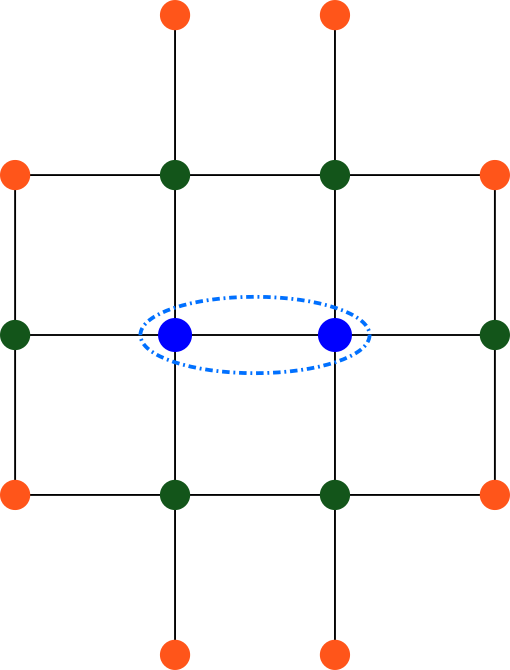
\includegraphics[width=0.3\textwidth]{dimer-nn.png}
	\caption{Blue circles indicate the dimer sites (enclosed by dotted circle). Green circles are the sites that are nearest neighbour to the dimer and the ones that are being summed over under the index \(l\). Orange circles are sites that are \textit{not} nearest neighbour to the dimer.}
	\label{dimer-nn}
\end{figure}

The total  Hamiltonian for a particular dimer pair \((i,j)\) then looks like:
\begin{equation}\begin{aligned}
	\tilde H^D(i, j) &= \frac{1}{2(w-1)}\sum_{l \in \text{NN of (i,j)}} \left[H^D(i, j) - t^D \sum_{\sigma}\left(c^\dagger_{i\sigma}c_{l,\sigma} + c^\dagger_{j\sigma}c_{l,\sigma} + \text{h.c.}\right) + \sum_{\vec k}^{\text{eff. bath (i,j)}\atop{z = l}}\epsilon_{\vec k}\hat n_{\vec k}\right]\\
			 &= H^D(i, j) + \frac{1}{2(w-1)}\sum_{l \in \text{NN of (i,j)}}\left[- t^D \sum_\sigma\left(c^\dagger_{i\sigma}c_{l,\sigma} + c^\dagger_{j\sigma}c_{l,\sigma} + \text{h.c.}\right) + \sum_{\vec k,\sigma}^{\text{eff. bath (i,j)}\atop{z = l}}\epsilon_{\vec k}\hat n_{\vec k}\right]
\end{aligned}\end{equation}
We now translate this Hamiltonian over all nearest neighbour pairs on the lattice, and take the average:
\begin{equation}\begin{aligned}
	\label{H_tiled}
	\tilde H = \frac{2}{Nw}\sum_{\left<ij\right>}\frac{1}{2(w-1)}\sum_{l \in \text{NN of (i,j)}}\tilde H^D(i, j, l) = \frac{2}{N}U^D\sum_{i} \tau_{i \uparrow}\tau_{i \downarrow} - \frac{2}{Nw}\left(1 + \frac{Nw}{2}\right)t^D\sum_{\left<ij\right>}\left(c^\dagger_{i\sigma}c_{j\sigma} + \text{h.c.}\right)
\end{aligned}\end{equation}
% Note that this local Hamiltonian actually has all the hoppings of the full Hubbard model, but the correlation is present just on the sites \(i,j\). We havent transformed the dimer parameters \(U^D, t^D\) to the Hubbard parameters yet.
% \\\\
% If we now sum over all the nearest-neighbour pairs and take the average of all the Hamiltonians (\(\frac{1}{2}Nw\) in number), we get
% \begin{equation}\begin{aligned}
% 	\tilde H &= \frac{2}{Nw}\sum_{\left<ij \right>}^N H^D_{i,j} \\
% 		 &= -t^A\sum_{\left<ij\right>}\left( c^\dagger_{i\sigma}c_{j\sigma} + \text{h.c.} \right) + \frac{2}{N}\sum_i U \tau_{i \uparrow}\tau_{i \downarrow}\\
% 		 &= \frac{1}{Nw}\left[\sum_{\sigma, i=1}^N\sum_{j \in \text{NN of }j}-t^D\left(c^\dagger_{\sigma}c_{j\sigma} + \text{h.c.}\right) + w U^D\sum_{i=1}^N \hat \tau_{i \uparrow}\hat \tau_{i \downarrow} + U^D\sum_{i=1}^N\sum_{j \in \text{N.N. of }i}\hat \tau_{j \uparrow}\hat \tau_{j \downarrow}\right]\\
% 		      &= \frac{1}{Nw}\left[-t^D 2\sum_{\sigma, \left<ij\right>}\left(c^\dagger_{\sigma}c_{j\sigma} + \text{h.c.}\right) + 2 U^D\sum_{\left<ij\right>} \hat \tau_{i \uparrow}\hat \tau_{i \downarrow} + 2 U^D\sum_{\left<ij\right>} \hat \tau_{j \uparrow}\hat \tau_{j \downarrow}\right]\\
% 		      &= \frac{2}{Nw}\sum_{\left<ij\right>}\left[-t^D \sum_\sigma \left(c^\dagger_{\sigma}c_{j\sigma} + \text{h.c.}\right) + U^D\left(\hat \tau_{i \uparrow}\hat \tau_{i \downarrow} + \hat \tau_{j \uparrow}\hat \tau_{j \downarrow}\right)\right]\\
% 		      &= \frac{2}{Nw}\sum_{\left<ij \right>} H^D(i,j,t^D, U^D)
% \end{aligned}\end{equation}
% There we used the identity
% \begin{equation}\begin{aligned}
% 	\sum_{i=1}^N\sum_{j \in \text{NN of }j} = 2\sum_{\left<ij\right>}
% \end{aligned}\end{equation}
The sum $\left<ij\right>$ is over all nearest-neighbour pairs. 
% Thus, $\tilde H$ can be written as
% \begin{equation}\begin{aligned}
% 	\label{H_tiled}
% 	\tilde H = - \frac{2t^D}{Nw}\sum_{\sigma, \left<ij \right>}\left(c^\dagger_{\sigma}c_{j\sigma} + \text{h.c.}\right) + \frac{2U^D}{N}\sum_i \hat \tau_{i \uparrow}\hat \tau_{i \downarrow} = \frac{2}{Nw}\sum_{\left<ij \right>} H^D(i,j,t^D, U^D)
% \end{aligned}\end{equation}
The conclusion is that on tiling the Hubbard dimer+bath Hamiltonians into all the nearest neighbour pairs, we end up with a new Hubbard model Hamiltonian with "renormalised parameters" given by
\begin{equation}\begin{aligned}
	\tilde t = \frac{2}{Nw}(1 + \frac{Nw}{2})t^D, &&\tilde U = \frac{2}{N}U^D
\end{aligned}\end{equation}
It is thus apparent that translating the Hubbard dimers throughout the lattice has restored translational invariance, and generated correlations on all sites. 
%(as compared to just on the impurity site). %This also takes care of the problem that the spectrum of the Anderson molecule and Hubbard dimer are different for the $N=1$ or $N=3$ sectors: By translating the Anderson molecule suitably, we have recovered the correct spectrum in all sectors.
% \\\\
% The claim made in a previous section was that this Hamiltonian is very close to a similarity transformed Hubbard Hamiltonian:
% \begin{equation}\begin{aligned}
% 	\tilde{H} = \frac{2}{Nw}\sum_{\left<ij \right>} H^D(i,j,t^D, U^D) \equiv  \mathcal{U} H^H  \mathcal{U}^{-1}~,
% \end{aligned}\end{equation}
% where $\mathcal{U}$ is in general distinct from the unitary transformation that completes the URG starting from the bare cluster+bath Anderson model up to the fixed-point Hamiltonian. As shown earlier, $U$ transformation that involves three steps: the URG transformations $\mathcal{U}_A$, the extracting of the zero mode $Z$ and the tiling procedure outline in this section, $T$
% \begin{equation}\begin{aligned}
% 	\mathcal{U} = T Z \mathcal{U}_{A}~.
% \end{aligned}\end{equation}
With some knowledge of the RG procedure, one can even write down the relation between the Hubbard dimer couplings $t^D, U^D$ and the parent Hubbard model parameters $t^H, U^H$. We have seen previously in another work that in the absence of any explicit spin or charge isospin exchange couplings, the impurity-bath hybridisation coupling $t^A$ does not flow under the RG. In going from the Hubbard model to the auxiliary model, we replace the non-local operator $c_i$ with the local operator $c_d$. If we define the normalization of the Fourier transform such that both spaces have $\frac{1}{\sqrt N}$, then the auxiliary model coupling can be written as $t^A = \sqrt N t^H$. When we write the fixed-point hopping purely in terms of zero mode, another such factor appears: $\sum_k c_k = \sqrt N c_0$, such that $t^D = \sqrt N (t^A)*$. Combining these, we get
\[ t^D = \sqrt N \times (t^A)^* = \sqrt N \times t^A = N \times t^H \]
As for the on-site repulsion $U^H$, we will constrain the RG flows such that the fixed-point value of the impurity ons-te repulsion $U^A$ is identical to that of the on-site repulsion of the bath, $U_b$. A sensible choice for the bath on-site repulsion is simply $U^H\times N$. The factor of $N$ maintains the extensivity of the bath correlation term. We can therefore write
\[U^D \equiv (U^A)* = U_b = N \times U^H\]
\section{Formal expressions for single particle Greens functions and other related many-body quantites}
\subsection{Expressing matrix elements of the inverse single particle Greens function in terms of Hubbard dimer counterparts}
%If the groundstate wavefunction of $H^H$ is $\ket{0}$, then the groundstate wavefunction of $\tilde H$ is $\ket{\tilde 0} =  \mathcal{U}\ket{0}$. The advantage of $\tilde H$ being connected to $H^H$ through unitary (or atleast similarity) transformations is that they will have the same single-particle Greens functions
%\begin{equation}\begin{aligned}
%	\left(G_H\right)^\sigma_{\nu \nu^\prime}(t) \equiv -i\theta(t)\bra{0}\left\{c_{\nu},c^\dagger_{\nu^\prime} \right\}\ket{0} &= -i\theta(t)\bra{0} \mathcal{U}^{-1}\left\{  \mathcal{U} c_{\nu}  \mathcal{U}^{-1}  \mathcal{U} c^\dagger_{\nu^\prime}  \mathcal{U}^{-1} +  \mathcal{U} c^\dagger_{\nu^\prime}  \mathcal{U}^{-1}  \mathcal{U} c_{\nu}  \mathcal{U}^{-1}\right\} \mathcal{U}\ket{0}\\
%															&=-i\theta(t)\bra{\tilde 0}\left\{\tilde c_{\nu} \tilde c^\dagger_{\nu^\prime} + \tilde c^\dagger_{\nu^\prime} \tilde c_{\nu} \right\}\ket{\tilde 0}\\
%															&= \left(\tilde G\right)_{\tilde {\nu} \tilde {\nu^\prime}}(t)~.
%\end{aligned}\end{equation}
%This says that the Greens function $G_H$ of the bare Hubbard model $H^H$ for propagation of excitations (on top of its ground state $\ket{0}$) starting from $\ket{\nu^\prime} \equiv c^\dagger_{\nu^\prime}\ket{0}$ and ending at $\ket{\nu} \equiv c^\dagger_{\nu}\ket{0}$ is exactly equal to the Greens function $\tilde G$ of the renormalised Hamiltonian $\tilde H$ for propagation of the renormalised excitations (on top of its renormalised ground state $\ket{\tilde 0} =  \mathcal{U} \ket{0}$) starting from $\ket{\tilde {\nu^\prime}} \equiv \tilde c^\dagger_{\nu^\prime}\ket{\tilde 0} \equiv  \left(\mathcal{U} c^\dagger_{\nu^\prime}  \mathcal{U}^{-1}\right)  \mathcal{U}\ket{0} =  \mathcal{U}\ket{{\nu^\prime}}$ and ending at $\ket{\tilde \nu} \equiv \tilde c^\dagger_{\nu}\ket{\tilde 0}$. This means,
%\begin{equation}\begin{aligned}
%	\bra{\nu}G_H\ket{{\nu^\prime}} = \bra{\tilde {\nu}}\tilde G\ket{\tilde {\nu^\prime}}
%\end{aligned}\end{equation}
Since the two Hamiltonians $H^H$ and $\tilde H$ are connected via a similarity transformation $\mathcal{U}$, their ground states are also connected by the same transformation. That is, if the ground states are $\ket{\Phi_0}$ and $\ket{\tilde{\Phi_0}}$ respectively, then $\ket{\tilde{\Phi_0}} = \mathcal{U}\ket{\Phi_0}$. This means that matrix elements of the type in eq.~\ref{G_mat_el} will also be connected. The matrix elements are of the inverse Greebs function operator defined in eq.~\ref{inv_G_func}:
 \begin{equation}\begin{aligned}
	 \mathcal{G}(\omega, H) = \frac{1}{\omega - (H - E_\text{GS})}
 \end{aligned}\end{equation}
Its easy to see that the matrix elements of the original and renormalised versions of this operator, between the original and renormalised states, are equal:
\begin{equation}\begin{aligned}
	\left[\mathcal{G}_H^{-1}\right]_{\nu \nu^\prime} = \bra{\nu}\omega - H^H + E_\text{GS}\ket{\nu^\prime} = \bra{\nu} \mathcal{U}^{-1}\left(\omega -  \mathcal{U} H^H  \mathcal{U}^{-1} + E_\text{GS}\right)  \mathcal{U}\ket{\nu^\prime} = \bra{\tilde \nu}\left(\omega - \tilde H + E_\text{GS}\right)\ket{\tilde \nu^\prime}\\
	= \left[\mathcal{\tilde G}^{-1}\right]_{\tilde \nu,\tilde \nu^\prime}
\end{aligned}\end{equation}
where we have defined the renormalised excitation $\ket{\tilde {\nu^\prime}} \equiv \tilde c^\dagger_{\nu^\prime}\ket{\tilde \Phi_0} \equiv  \left(\mathcal{U} c^\dagger_{\nu^\prime}  \mathcal{U}^{-1}\right)  \mathcal{U}\ket{\Phi_0} =  \mathcal{U}\ket{{\nu^\prime}}$. These equalities are important because they allows us to calculate these matrix elements for $\tilde H$ and then equate them to those of $H^H$, and once we have the matrix elements of $\mathcal{G}$, we can use them to obtain the single-particle Greens functions using eq.~\ref{G_mat_el}. More specifically, to calculate the real space single-particle Greens function between the lattice sites $i$ and $j$, both with spin $\sigma$, we will use the relation:
\begin{equation}\begin{aligned}
	G(i\sigma, j\sigma, \omega) = \bra{ i\sigma} \mathcal{G}(\omega, H) \ket{ j\sigma} - \bra{\overline{i\sigma}} \mathcal{G}(-\omega, H) \ket{\overline {j\sigma}} = \mathcal{G}(\omega, H)_{ i\sigma, j\sigma} - \mathcal{G}(-\omega, H)_{\overline{i\sigma}, \overline {j\sigma}}
\end{aligned}\end{equation}
where $\ket{i\sigma}=c^\dagger_{i\sigma}\ket{\Phi_0}$ and $\ket{\overline{i\sigma}}=c_{i\sigma}\ket{\Phi_0}$. We can see from the relation that we will need two types of matrix elements, one that propagates a particle excitation $\left( \ket{i\sigma} \right) $ and the one that propagates a hole excitation $\ket{\overline{i\sigma}}$.
\\\\
To this end, we rewrite eq.~\ref{H_tiled} in terms of inverse Greens function operators for the new (symmetrized) Hubbard model and the Hubbard dimer respectively:
\begin{equation}\begin{aligned}
	\label{Gd_op}
	\mathcal{\tilde G}(\omega) = \frac{1}{\omega - \left(\tilde H - E_\text{GS}\right)}, && \mathcal{G}_D(\omega) = \frac{1}{\omega - \left(\tilde H^D(i,j,l) - E_\text{GS}\right)}
\end{aligned}\end{equation}
%\textit{It has been assumed that the Hamiltonians have been normal ordered such that the ground state energy is 0.} Then, these are the same operators that appear in the appendix.
These are the same operators that appear in the appendix. However, before proceeding, we should note that even though eq.~\ref{H_tiled} used the indices $i,$, the correct indices are actually $\tilde i, \tilde j$, in light of the fact that operators get renormalised as $c_i \to \tilde c_i\equiv Uc_i$. With this in mind, we can write
\begin{equation}\begin{aligned}
	\label{green_eq}
	\omega - \mathcal{\tilde G}^{-1}(\omega) = \frac{2}{Nw}\sum_{\left<\tilde i, \tilde j\right>} \frac{1}{2(w-1)} \sum_{l \in \text{NN of j}}\left[\omega - \mathcal{G}_D^{-1}\left(\tilde i, \tilde j, \tilde l\right)\right]
\end{aligned}\end{equation}
where $\mathcal{G}_D^{-1}(\tilde i,\tilde j, \tilde l)$ is the Greens function inverse matrix of the Hubbard dimer+bath Hamiltonian with $\tilde i, \tilde j$ as the two sites and \(\tilde l\) as the zero mode of the bath, eq.~\ref{Hdjl}, or equivalently, eq.~\ref{dimer_p_bat}. Since the $\omega$ on the RHS of eq.~\ref{green_eq} is independent of the summation indices, they can be pulled out along with a factor. The factor is just the total number of nearest neighbour pairs, which is $\frac{Nw}{2}$. This allows it to cancel the $\omega$ on the LHS. The equation then simplifies to
\begin{equation}\begin{aligned}
	\mathcal{\tilde G}^{-1}(\omega) = \frac{2}{Nw}\sum_{\left<i,j\right>}\frac{1}{2(w-1)}\sum_{l \in \text{NN of j}}\mathcal{G}_D^{-1}\left(\omega, \tilde i, \tilde j, \tilde l\right)
\end{aligned}\end{equation}
Because of translational invariance, all values of \(l\) should give the same Greens function, and we can simplify this to
\begin{equation}\begin{aligned}
	\label{green_eq_final}
	\mathcal{\tilde G}^{-1}(\omega) = \frac{2}{Nw}\frac{1}{2(w-1)}\times 2(w-1)\sum_{\left<i,j\right>}\mathcal{G}_D^{-1}\left(\omega, \tilde i, \tilde j\right) = \frac{2}{Nw}\sum_{\left<i,j\right>}\mathcal{G}_D^{-1}\left(\omega, \tilde i, \tilde j\right)
\end{aligned}\end{equation}
We dropped the index \(\tilde l\) on \(\mathcal{G}_D^{-1}\) to mean that any particular choice of \(\tilde l\) will do. We will now calculate the site-diagonal and site-off-diagonal matrix elements for particle propagation. The site-diagonal matrix element will be calculated between the state $\ket{\tilde i, \sigma} = \mathcal{U}c^\dagger_{i\sigma}\ket{\Phi_0}$ and its bra, while the off-diagonal one is between $\ket{\tilde j\sigma}$ and $\bra{\tilde i\sigma}$. Since it has already been shown that the matrix elements of the renormalised Hamiltonian are the same as those of the original Hamiltonian, we will directly replace the former with the latter. \\\\
First lets consider the diagonal matrix element at $\tilde i^\text{th}$ site. The only terms that will contribute on the RHS of eq.~\ref{green_eq_final} are those that have the index $\tilde i$ on the dimer. There are $w$ terms that have the index \(\tilde i\) on the dimer corresponding to the $w$ nearest neighbours of \(\tilde i\). Thus, the right hand side will be a sum of $w$ terms, each term being the inverse Greens function of a Hubbard dimer+bath Hamiltonian. Each term will be a real space local Greens function, and because of translational invariance, it will be the same for all choices of the nearest neighbour of \(\tilde i\). %So we will represent the real space local inverse Greens function as $\left[\mathcal{G}_D^{-1}(\omega)\right]_{00}^{\sigma}$.
% \begin{gather}
% 	\label{local_gf}
% 	\left(\mathcal{G}_{H}^{-1}(\omega)\right)_{ii}^\sigma = \frac{2}{Nw}\left[\mathcal{G}_{D}^{-1}(\omega)\right]^\sigma_{00}\times w = \frac{2}{N}\left[\mathcal{G}_{D}^{-1}(\omega)\right]^\sigma_{00} \equiv g_0\\
% 	\left[\mathcal{G}_{D}^{-1}(\omega)\right]^\sigma_{00} = \bra{\Phi_0}c_{0\sigma}\mathcal{G}_{D}^{-1}(\omega)c^\dagger_{0\sigma}\ket{\Phi_0}
% \end{gather}
\begin{gather}
	\left(\mathcal{G}_{H}^{-1}(\omega)\right)_{ii}^\sigma = \frac{2}{Nw}\sum_{j \in \text{NN of i}}\bra{\tilde \Phi_0}c_{i\sigma}\mathcal{G}_{D}^{-1}(\omega, \tilde i, \tilde j)c^\dagger_{i\sigma}\ket{\tilde \Phi_0} = \frac{2}{N}\bra{\tilde \Phi_0}c_{i\sigma}\mathcal{G}_{D}^{-1}(\omega, \tilde i)c^\dagger_{i\sigma}\ket{\tilde \Phi_0}
\end{gather}
Once we have stripped away the \(j,l\) dependence, we can view the RHS as simply the matrix element of the dimer-bath Hamiltonian eq.~\ref{dimer_p_bat} between the local states of the site zero of the bath:
\begin{gather}
	\label{local_gf}
	\left(\mathcal{G}_{H}^{-1}(\omega)\right)_{ii}^\sigma = \frac{2}{N}\bra{\tilde \Phi_0}c_{0\sigma}\mathcal{G}_{D}^{-1}(\omega)c^\dagger_{0\sigma}\ket{\tilde \Phi_0}
\end{gather}
Just to make it explicit, we repeat once more that \(\mathcal{G}_{D}^{-1}(\omega)\) is the inverse Greens function operator of the Hamiltonian in eq.~\ref{dimer_p_bat}.
We can expand the state $c^\dagger_{i\sigma}\ket{\tilde \Phi_0}$ in terms of a complete set of orthogonal states:
\begin{equation}\begin{aligned}
	c^\dagger_{0\sigma}\ket{\tilde \Phi_0} = \sum_n C^0_n \ket{n}, && c^\dagger_{1\sigma}\ket{\tilde \Phi_0} = \sum_n C^1_n \ket{n}%\sum_{m,\alpha,\beta} C^i_{m,\alpha,\beta} \ket{m,\alpha,\beta}
\end{aligned}\end{equation}
where $C^{0}$ and $C^{1}$ are coefficients of the linear superposition defined by
\begin{equation}
C^{0}_{n} = \bra{n} c^\dagger_{0\sigma}\ket{\tilde \Phi_0}~,~ C^{1}_{n} = \bra{n} c^\dagger_{1\sigma}\ket{\tilde \Phi_0}~.
\end{equation}
Due to the translation invariance, the coefficients $C^{0}_{n}$ and $C^{1}_{n}$ are independent of the site indices. The index $n$ actually defines a set of quantum numbers that characterize the state $\ket{n}$. For example it might be a combination of number of particles, parity and total spin angular momentum $(n \equiv n, P, S^z)$. In light of the Greens function we have in between te states, we choose the orthogonal set to be formed by the eigenstates of the dimer+bath Hamiltonian.
% One simple way of choosing the orthogonal basis $\left\{ \ket{n} \right\}$ is to take them from the eigenstates of a system comprising a Hubbard dimer and a conduction bath, decoupled from each other. The dimer will of course have 2 sites, which means the conduction bath will have $N-2$ sites, or $N-2$ momentum states. The set of eigenstates that have the total number of particles (combining the dimer and the bath) equal to $N+1$ will then form the basis in question. Since the dimer is decoupled from the bath, the total wavefunction will be a direct product of a Hubbard dimer wavefunction and a bath wavefunction.
% \begin{equation}\begin{aligned}
% 	\ket{m,\alpha,\beta} = \Phi^D_{m,\alpha} \otimes \Psi^B_{N-m+1, \beta}
% \end{aligned}\end{equation}
% $\alpha$ is an internal quantum number of the Hubbard dimer while $\beta$ is that for the bath. The subscripts $m$ and $N-m+1$ label the total number of particles in each part of the wavefunction. These two labels have to add to $N+1$. Our choice of the $\ket{n}$ is motivated by noting that the effective auxiliary model we are invoking here is that of a Hubbard dimer connected to a bath via single-particle hybridisation; the eigenstates of the isolated dimer and bath subsystems then act as the natural choices of the orthogonal bases in which to expand the wavefunction for the single-particle excitation of the interacting system $c^\dagger_{0\sigma}\ket{\tilde \Phi_0}$. Further, while the eigenstates ($\Phi^D_{m,\alpha}$) of the Hubbard dimer are known analytically, we can safely assume the eigenstates of the bath ($\Psi^B_{N-m+1, \beta}$) to be a simple direct product of various single-particle Fock states in $k$-space. We then compute the matrix element of eq.\eqref{local_gf} for site $i$ and its immediate neighbours (i.e., a given realisation of a auxiliary model). Then, using translation invariance, we demand that this matrix element is independent of the site index $i$. The correctness of this auxiliary model approach hinges on how close the state $\ket{\tilde{\Phi_0}}$ is to the 2-site local nature of the exact ground state of the target model (here the Hubbard model on a given lattice). Further improvement can be made by improving (i) the state $\ket{\tilde{\Phi_0}}$ for the present auxiliary model (involving a Hubbard dimer), or (ii) choosing a better auxiliary model with an ``impurity" system that has more sites than two (i.e., a Bethe-Peierls improvement of the dimer auxiliary model).
% \\\\
Using this expansion, the matrix element of $\mathcal{G}$ can be written as
\begin{equation}\begin{aligned}
	\left(\mathcal{G}_{H}^{-1}(\omega)\right)_{ii}^\sigma = \frac{2}{N}\sum_{nn^\prime} \left(C^0_{n^\prime}\right)^*\bra{n^\prime}\mathcal{G}_{D}^{-1}(\omega)\ket{n} C^0_{n}
\end{aligned}\end{equation}
Since $\ket{n}$ is an actual eigenstate of the Hamiltonian that defines \(\mathcal{G}_{D}^{-1}(\omega)\), $\mathcal{G}_{D}^{-1}(\omega)$ will be diagonal in that basis:
\begin{equation}\begin{aligned}
	\left(\mathcal{G}_{H}^{-1}(\omega)\right)_{ii}^\sigma = \frac{2}{N}\sum_{n} |C^0_{n}|^2 \left(\mathcal{G}_{D}^{-1}(\omega)\right)_{n n} 
\end{aligned}\end{equation}
Now we come to the off-diagonal Greens function for the nearest neighbour sites $i$ and $j$. This will receive contribution from only that dimer+bath Hamiltonian that has \(i,j\) as the dimer sites. This will not be a real space diagonal Greens function. Instead, it involves two nearest neighbour sites. %We call this Greens function $\left[\mathcal{G}_D^{-1}(\omega)\right]_{01}^\sigma$.
\begin{gather}
\label{nn_gf}
\left(\mathcal{G}_{H}^{-1}(\omega)\right)_{ij}^\sigma = \frac{2}{Nw}\bra{\tilde \Phi_0}c_{0\sigma}\mathcal{G}_{D}^{-1}(\omega)c^\dagger_{1\sigma}\ket{\tilde \Phi_0} = \frac{2}{Nw}\sum_{n} \left(C^0_{n}\right)^* C^1_{n} \left(\mathcal{G}_{D}^{-1}(\omega)\right)_{nn} 
%\left(\mathcal{G}_{H}^{-1}(\omega)\right)_{ij}^\sigma = \frac{2}{Nw}\left[\mathcal{G}_{D}^{-1}(\omega)\right]_{01}^\sigma \equiv g_1\\
	%\left[\mathcal{G}_{D}^{-1}(\omega)\right]^\sigma_{01} = \bra{\Phi_0}c_{0\sigma}\mathcal{G}_{D}^{-1}(\omega)c^\dagger_{1\sigma}\ket{\Phi_0}
\end{gather}
For convenience, we define $g_n = \left(\mathcal{G}_{D}^{-1}(\omega)\right)_{nn}$.
\begin{figure}[htpb!]
	\centering
	\hspace*{\fill}
	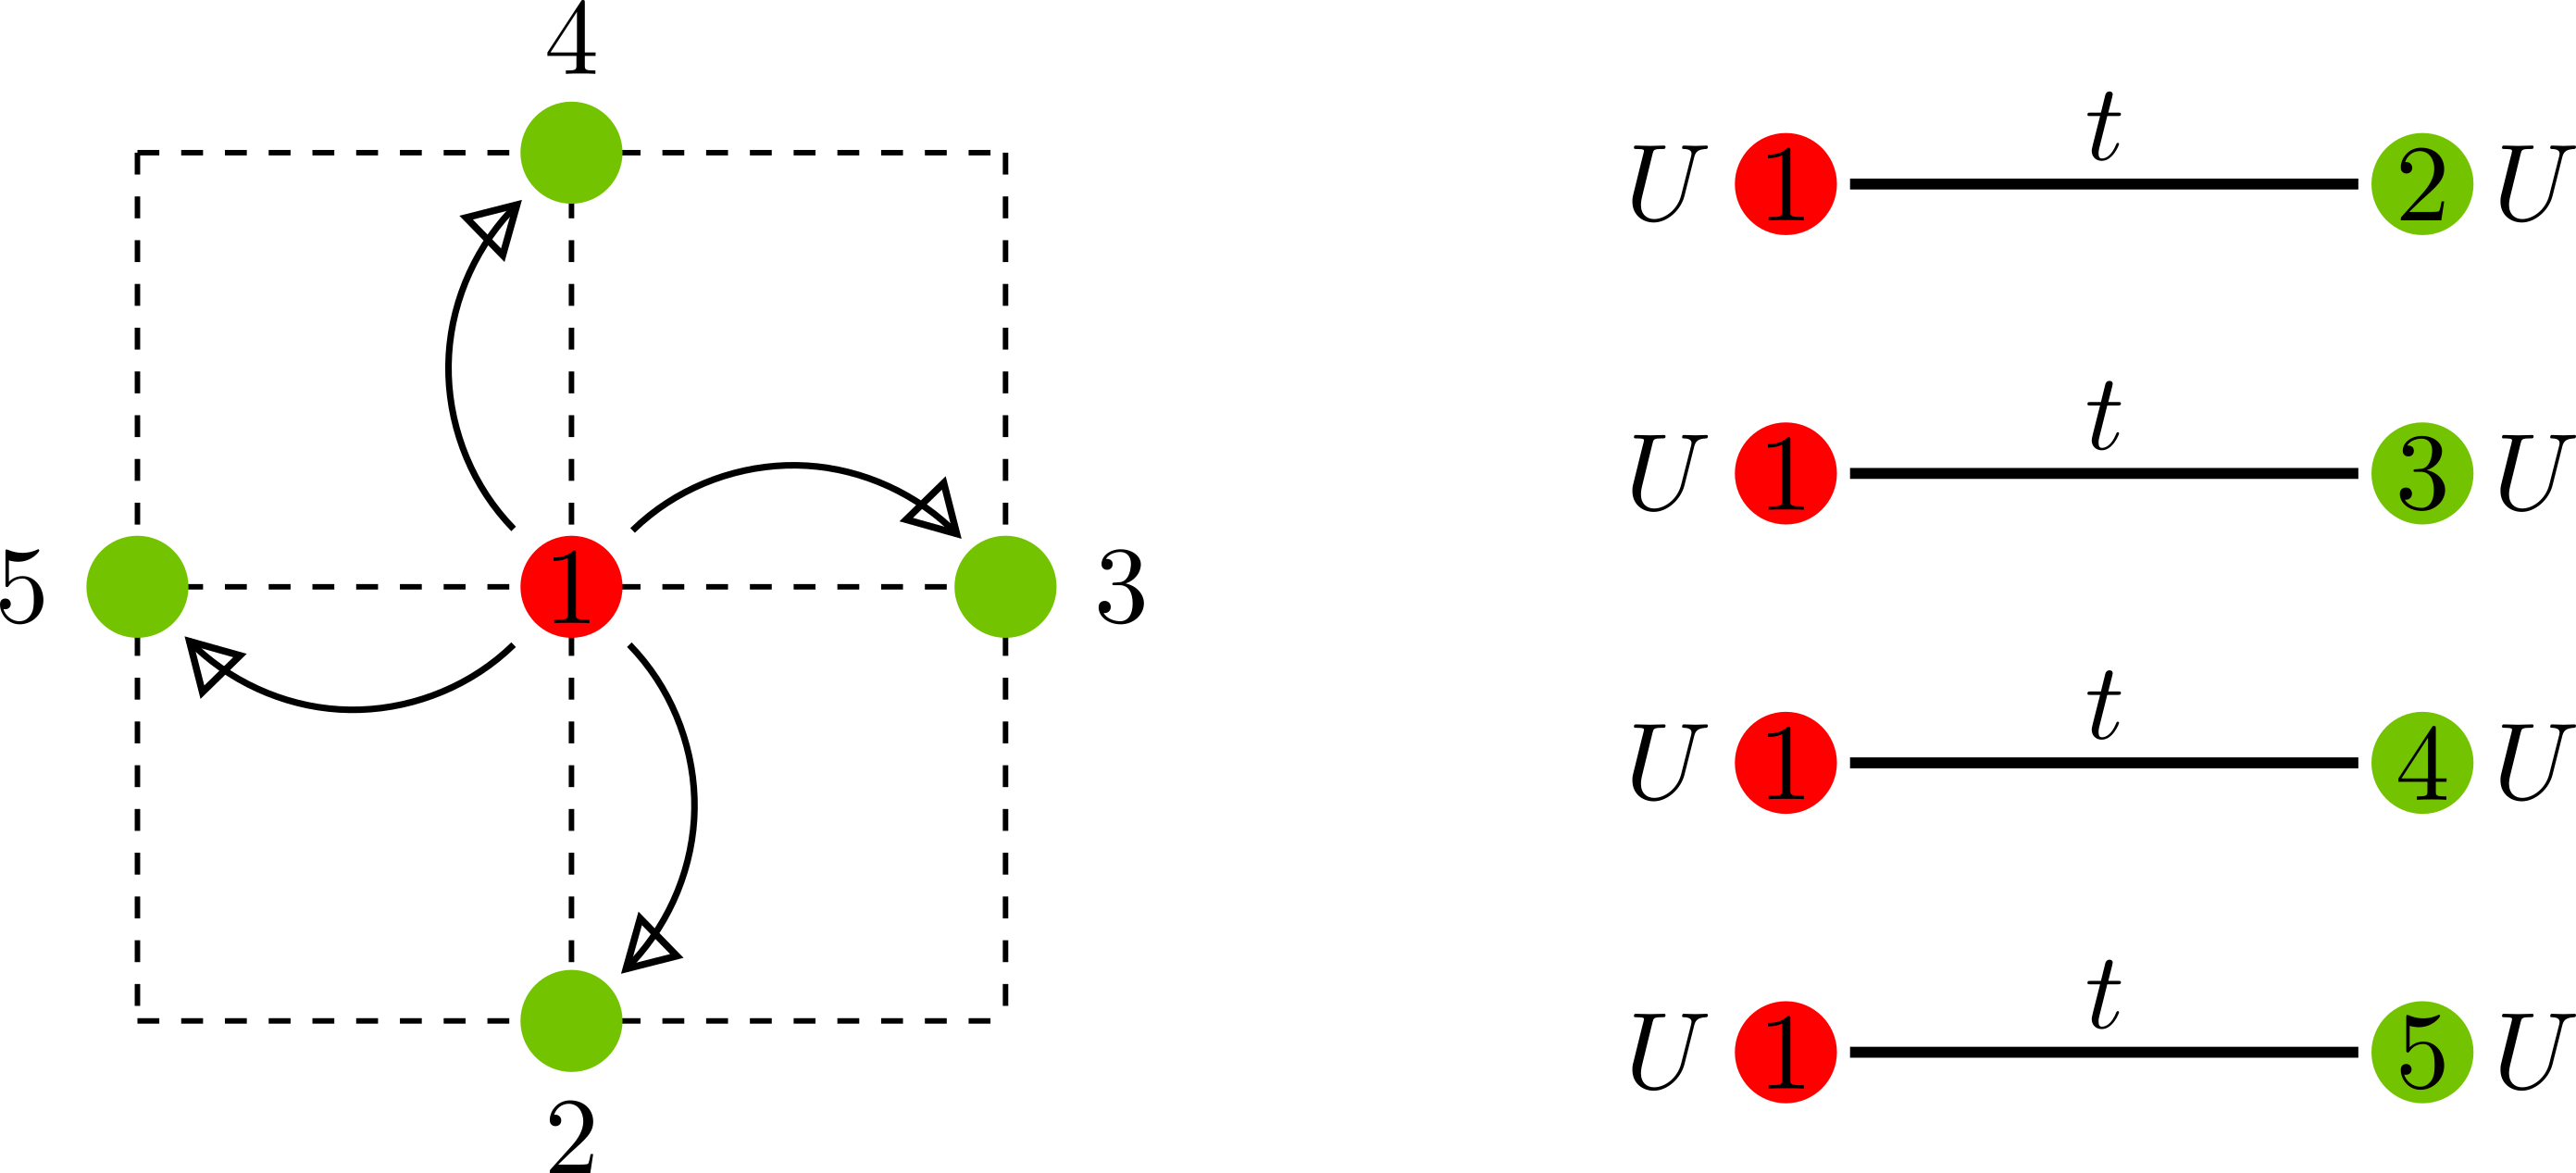
\includegraphics[width=0.7\textwidth]{lattice.png}
	\hspace*{\fill}
	\caption{\textit{Left:} Part of the lattice that is picked out by the Greens function on the LHS of eq.~\ref{local_gf}. \textit{Right:} Hamiltonian whose Greens functions appear on the right hand side of same equation. The two submodels are identical.}
\end{figure}
\\\\
The matrix elements for hole propagation are obtained similarly. Here the relavant excitations are $\ket{\overline{i\sigma}} \equiv c_{i\sigma}\ket{\tilde \Phi_0}$, at frequency $-\omega$. To expand these states, we choose the eigenstates with $N-1$ total particles as the orthonormal basis:
\begin{equation}\begin{aligned}
	c_{0\sigma}\ket{\tilde \Phi_0} = \sum_n \overline C^0_n \ket{\overline{n}}, && c_{1\sigma}\ket{\tilde \Phi_0} = \sum_n \overline C^1_n \ket{\overline{n}}%\sum_{m,\alpha,\beta} C^i_{m,\alpha,\beta} \ket{m,\alpha,\beta}
\end{aligned}\end{equation}
and the counterpart for $g_n$, here, is
\begin{equation}\begin{aligned}
	\overline {g_n} = \bra{\overline n}\mathcal{G}_{D}^{-1}(-\omega)\ket{\overline n}
\end{aligned}\end{equation}
By suitably replacing the symbols, we can write down the matrix elements of $\mathcal{G}_H^{-1}(-\omega)$ for hole propagation:
\begin{equation}\begin{aligned}
	\left(\mathcal{G}_{H}^{-1}(-\omega)\right)_{\overline{ii}}^\sigma &= \frac{2}{N}\sum_{n} |\overline C^0_{n}|^2 \overline{g_n}\\
	\left(\mathcal{G}_{H}^{-1}(-\omega)\right)_{ij}^\sigma &= \frac{2}{Nw}\sum_{n} \left(\overline C^0_{n}\right)^* \overline C^1_{n} \overline{g_n} 
\end{aligned}\end{equation}


% \begin{equation}\begin{aligned}
% 	\label{hole_gf}
% 	&\left(\mathcal{G}_{H}^{-1}(-\omega)\right)_{\overline{ii}}^\sigma = \frac{2}{N}\left[\mathcal{G}_{D}^{-1}(-\omega)\right]^\sigma_{\overline{00}} \equiv \overline{g_0}, &&&\left[\mathcal{G}_{D}^{-1}(-\omega)\right]^\sigma_{\overline{00}} = \bra{0}c^\dagger_{0\sigma}\mathcal{G}_{D}^{-1}(-\omega)c_{0\sigma}\ket{0}\\
% 	&\left(\mathcal{G}_{H}^{-1}(-\omega)\right)_{\overline{ij}}^\sigma = \frac{2}{Nw}\left[\mathcal{G}_{D}^{-1}(-\omega)\right]_{\overline{01}}^\sigma \equiv \overline{g_1}, &&&\left[\mathcal{G}_{D}^{-1}(-\omega)\right]^\sigma_{\overline{01}} = \bra{0}c^\dagger_{0\sigma}\mathcal{G}_{D}^{-1}(-\omega)c_{1\sigma}\ket{0}
% \end{aligned}\end{equation}

\subsection{Constructing full Greens function matrix from the inverse matrix}
The matrix elements $\left(\mathcal{G}_{H}^{-1}(\omega)\right)_{ii}^\sigma$ and its nearest neighbour partner can be obtained simply by inverting the internal matrix $\mathcal{G}^{-1}_D$. This is because,
\begin{equation}\begin{aligned}
	A_{ij} = \sum_{mn}\braket{i | n} A_{nm} \braket{m|j} \implies A^{-1}_{ij} = \sum_{mn}\braket{i|n} A^{-1}_{nm} \braket{m|j}
\end{aligned}\end{equation}
The spectral weights remain unchanged; only the matrix element changes from $A_{nm}$ to $(A^{-1})_{nm}$. Inverting the matrix $\mathcal{G}_D$ is actually simple because it is diagonal in the chosen basis:
\begin{equation}\begin{aligned}
	\left(\mathcal{G}^{-1}_D\right)_{nn} = \begin{pmatrix} g_{0} && 0 && &..& 0\\ 0 && g_{1} && && \\ &&..&& .. &&  \\ 0 &&&&&& g_{M} \end{pmatrix} \implies \left(\mathcal{G}_D\right)_{nn} = \begin{pmatrix} \frac{1}{g_{0}} && 0 && &..& 0\\ 0 && \frac{1}{g_{1}} && && \\ &&..&& .. &&  \\ 0 &&&&&& \frac{1}{g_{M}} \end{pmatrix}
\end{aligned}\end{equation}
This allows us to write
\begin{equation}\begin{aligned}
	\label{G_mat_loc}
	\left(\mathcal{G}_{H}(\omega)\right)_{ii}^\sigma = \frac{4(w-1)}{N}\sum_{n} |C^0_{n}|^2 \frac{1}{g_n}, && \left(\mathcal{G}_{H}(-\omega)\right)_{\overline{ii}}^\sigma = \frac{4(w-1)}{N}\sum_{n} |\overline C^0_{n}|^2 \frac{1}{\overline{g_n}}
\end{aligned}\end{equation}
and
\begin{equation}\begin{aligned}
	\label{G_mat_nn}
	\left(\mathcal{G}_{H}(\omega)\right)_{ij}^\sigma = \frac{4(w-1)}{Nw}\sum_{n} {C^0_{n}}^* C^1_{n} \frac{1}{g_n}, && \left(\mathcal{G}_{H}(-\omega)\right)_{\overline{ij}}^\sigma = \frac{4(w-1)}{Nw}\sum_{n} {\overline C^0_{n}}^* \overline C^1_{n} \frac{1}{\overline{g_n}}
\end{aligned}\end{equation}
These two expressions can be used to obtain an expression for the real space local and nearest-neighbour Greens functions:
\begin{equation}\begin{aligned}
	G_H(\omega)_\text{loc} &= \left(\mathcal{G}_H(\omega)\right)_{ii} - \left(\mathcal{G}_H(-\omega)\right)_{\overline{ii}} = \frac{4(w-1)}{N}\sum_n\left(|C^0_{n}|^2 \frac{1}{g_n} - |\overline C^0_{n}|^2 \frac{1}{\overline{g_n}}\right)\\
	G_H(\omega)_\text{nn} &= \left(\mathcal{G}_H(\omega)\right)_{ij} - \left(\mathcal{G}_H(-\omega)\right)_{\overline{ji}} = \frac{4(w-1)}{Nw}\sum_n\left({C^0_{n}}^* C^1_{n} \frac{1}{g_n} - {\overline C^0_{n}}^* \overline C^1_{n} \frac{1}{\overline{g_n}}\right)\\
\end{aligned}\end{equation}
The momentum space Greens function can be expressed as a Fourier transform of the real space Greens functions:
\begin{equation}\begin{aligned}
	G_H (\vec k, \omega) = \frac{1}{N}\sum_{\vec r, \vec r_j}e^{i \vec{k}\cdot\left(\vec{r_i} - \vec {r_j}\right)}G_H (|\vec{r_i} - \vec {r_j}|, \omega)
\end{aligned}\end{equation}
where $\vec{r_i}$ is the position vector of a particular lattice site. Because of translation invariance, the real space Greens function depends only on the relative vector between any two sites. As a result, $\vec r=0$ gives the local Greens function, $|\vec r|=a$ gives the nearest-neighbour Greens function and so on ($a$ being the lattice spacing). As we do not have real space Greens function that are more non-local than nearest neighbour, we will attempt to obtain momentum space Greens function from these two contributions:
\begin{equation}\begin{aligned}
	G_H (\vec k, \omega) \simeq \frac{1}{N}\sum_{\vec{r_i} = \vec {r_j}}G_H (\omega)_\text{loc} + \frac{1}{N}\sum_{|\vec{r_i} - \vec {r_j}|=a} e^{i \vec{k}\cdot\left(\vec{r_i} - \vec {r_j}\right)}G_H (\omega)_\text{nn}
\end{aligned}\end{equation}
The first summation produces a factor of $N$, while the second summation can be factorized into a sum over all sites (which again returns $N$) and a sum over all the primitive vectors connecting any single site with all its nearest neighbours, $\left\{ \vec a_i: i \in \left[1, w\right]\right\}$.
\begin{equation}\begin{aligned}
	\label{k_Gf}
	G_H (\vec k, \omega) &\simeq G_H (\omega)_\text{loc} + G_H (\omega)_\text{nn}\sum_{i=1}^w e^{i \vec{k}\cdot\vec {a_i}}\\
			     &= G_H (\omega)_\text{loc} + G_H (\omega)_\text{nn} \xi_{\vec k}\\
			     &= \frac{4(w-1)}{N}\sum_n\left[\left(|C^0_{n}|^2 + \frac{\xi_{\vec{k}}}{w}{C^0_{n}}^* C^1_{n} \right)\frac{1}{g_n} - \left(|\overline C^0_{n}|^2 + \frac{\xi_{\vec{k}}}{w}{\overline C^0_{n}}^* \overline C^1_{n}\right)\frac{1}{\overline{g_n}}\right]
\end{aligned}\end{equation}
where we defined \(\xi_{\vec k} \equiv \sum_{i=1}^w e^{i \vec{k}\cdot\vec {a_i}}\). For example, on a d-dimensional hypercubic lattice, we obtain
\begin{equation}\begin{aligned}
	\xi_{\vec k} = \sum_{i=1}^d \left(e^{i k_i {a_i}} + e^{-i k_i {a_i}}\right) = 2\sum_{i=1}^d \cos k_i a_i
\end{aligned}\end{equation}
On a 2D square lattice with lattice spacing $a$, this simplifies to
\begin{eqnarray}
	\label{2dsquaretb}
\xi_{\vec{q}} &=& 2(\cos q_{x}a + \cos q_{y}a)\equiv \frac{-\epsilon_{\vec{q}}}{t^{H}}~,\nonumber\\
\epsilon_{\vec{q}} &=& -2t^{H}(\cos q_{x}a_{x} + \cos q_{y}a_{y})~
\end{eqnarray}
where \(\epsilon_{\vec{q}}\) is the tight-binding dispersion.
\\\\
We can now compute the $k$-space spectral function $A_{H}(\vec{k},\omega)$ and the real-space local spectral function $A_{H}(\vec{r}=0,\omega)$ as
\begin{equation}\begin{aligned}
	A_{H}(\vec{k},\omega) &= -\frac{1}{\pi} \textrm{Im}(G_{H}(\vec{k},\omega)) = -\frac{4(w-1)}{N\pi} \textrm{Im}\sum_n\left[\left(|C^0_{n}|^2 + \frac{\xi_{\vec{k}}}{w}{C^0_{n}}^* C^1_{n} \right)\frac{1}{g_n} - \left(|\overline C^0_{n}|^2 + \frac{\xi_{\vec{k}}}{w}{\overline C^0_{n}}^* \overline C^1_{n}\right)\frac{1}{\overline{g_n}}\right]\\
A_{H}(\vec{r}=0,\omega) &= -\frac{1}{\pi} \textrm{Im}(G_{H}(\vec{r}=0,\omega)) = \frac{1}{N}\sum_{\vec{k}}A_{H}(\vec{k},\omega)
\end{aligned}\end{equation}
We can again use eqs.\eqref{2dsquaretb}, \eqref{local_gf} and \eqref{nn_gf} to obtain the spectral functions  $A_{H} (\vec{k},\omega)$ and $A_{H} (\vec{r}=0,\omega)$ for the Hubbard model on the 2D square lattice.

% Since the only real-space interaction is that between the nearest neighbours, there are no further real space Greens functions. Because of translational invariance, we know that $\left(\mathcal{G}_H^{-1}\right)_{ii}$ and $\left(\mathcal{G}_H^{-1}\right)_{ij}$ are independent of $i,j$. Furthermore, all expressions below are for a particular spin $\sigma$; from the spin rotational symmetry of the Hubbard Hamiltonian, the same expressions are obtained for the opposite spin. We will now recreate the entire matrix $\mathcal{G_H}^{-1}$ using the matrix elements we calculated previously. Since the two sets $\left\{ \ket{i\sigma} \right\}$ and $\left\{ \ket{\overline{i\sigma}}\right\}$ are orthogonal, we will create separate matrix for the two sets.
% \begin{equation}\begin{aligned}
% 	\mathcal{G}^{-1}_H(\omega) = \begin{pmatrix} \left(\mathcal{G}^{-1}\right)_{00} & \left(\mathcal{G}^{-1}\right)_{01} & ... & ... & \left(\mathcal{G}^{-1}\right)_{0N}\\
% 		\left(\mathcal{G}^{-1}\right)_{10} & \left(\mathcal{G}^{-1}\right)_{11} & \left(\mathcal{G}^{-1}\right)_{12} & ... & ...\\
% 		... & \left(\mathcal{G}^{-1}\right)_{21} & \left(\mathcal{G}^{-1}\right)_{22} & \left(\mathcal{G}^{-1}\right)_{23} & ... \\
% 		    &&.&&\\
% \end{pmatrix} = \begin{pmatrix} g_0 & g_1 & ... & ... & g_1\\
% 		g_1 & g_0 & g_1 & ... & ...\\
% 		... & g_1 & g_0 & g_1 & ... \\
% 		    &&...&&\\
% \end{pmatrix}\\
% 		\overline{\mathcal{G}^{-1}_H}(-\omega) = \begin{pmatrix} \left(\mathcal{G}^{-1}\right)_{\overline{00}} & \left(\mathcal{G}^{-1}\right)_{\overline{01}} & ... & ... & \left(\mathcal{G}^{-1}\right)_{\overline{0N}}\\
% 			\left(\mathcal{G}^{-1}\right)_{\overline{10}} & \left(\mathcal{G}^{-1}\right)_{\overline{11}} & \left(\mathcal{G}^{-1}\right)_{\overline{12}} & ... & ...\\
% 			... & \left(\mathcal{G}^{-1}\right)_{\overline{21}} & \left(\mathcal{G}^{-1}\right)_{\overline{22}} & \left(\mathcal{G}^{-1}\right)_{\overline{23}} & ... \\
% 		    &&.&&\\
% 			\end{pmatrix} = \begin{pmatrix} \overline{g_0} & \overline{g_1} & ... & ... & \overline{g_1}\\
% 			\overline{g_1} & \overline{g_0} & \overline{g_1} & ... & ...\\
% 			... & \overline{g_1} & \overline{g_0} & \overline{g_1} & ... \\
% 		    &&...&&\\
% \end{pmatrix} 
% \end{aligned}\end{equation}
% Both the matrices can be written in the operator form of a tight-binding Hamiltonian:
% \begin{equation}\begin{aligned}
% 	\mathcal{G}_H^{-1}(\omega) = g_0\sum_{i=1}^N\ket{i}\bra{i} + g_1\sum_{\left<i,j \right>}^N\left( \ket{i}\bra{j} + \text{h.c.}\right)\\
% 	\overline{\mathcal{G}_H^{-1}}(-\omega) = \overline{g_0}\sum_{\overline i=1}^N\ket{\overline i}\bra{\overline i} + \overline{g_1}\sum_{\left<\overline i,\overline j \right>}^N\left( \ket{\overline i}\bra{\overline j} + \text{h.c.}\right)
% \end{aligned}\end{equation}
% We can Fourier transform the real space kets $\ket{i} \equiv \ket{\vec r_i}$ into momentum space:
% \begin{flalign*}
% 	\ket{\vec r_i} &\equiv c^\dagger_{\vec r_i\sigma}\ket{0} = \frac{1}{\sqrt N}\sum_{\vec k=\vec k_1}^{\vec k_N} e^{i \vec{k}\cdot\vec{r_i}}c^\dagger_{k\sigma}\ket{0} \equiv \frac{1}{\sqrt N}\sum_{\vec k=\vec k_1}^{\vec k_N} e^{i \vec{k}\cdot\vec{r_i}}\ket{\vec k} \Leftrightarrow \ket{k} = \frac{1}{\sqrt N}\sum_{\vec i} e^{-i \vec{k}\cdot\vec{r_i}}\ket{\vec r_i} \\
% 	\ket{\overline{\vec r_i}} &\equiv c_{\vec r_i\sigma}\ket{0} = \frac{1}{\sqrt N}\sum_{\vec k=\vec k_1}^{\vec k_N} e^{i \vec{k}\cdot\vec{r_i}}c_{k\sigma}\ket{0} \equiv \frac{1}{\sqrt N}\sum_{\vec k=\vec k_1}^{\vec k_N} e^{i \vec{k}\cdot\vec{r_i}}\ket{\overline{\vec k}} \Leftrightarrow \ket{\overline{\vec k}} = \frac{1}{\sqrt N}\sum_{\vec i} e^{-i \vec{k}\cdot\vec{r_i}}\ket{\overline{\vec r_i}}
% \end{flalign*}
% We will now Fourier transform the matrix $\mathcal{G}_H^{-1}(\omega)$ to momentum space. In doing so, we will diagonalize the matrix.
% \begin{flalign*}
% 	\sum_i \ket{i}\bra{i} &= \frac{1}{N}\sum_i \sum_{\vec k, \vec q} e^{i \left(\vec{k} - \vec q\right)\cdot\vec{r_i}}\ket{\vec k}\bra{\vec q} = \frac{1}{N}\sum_{\vec k, \vec q} N \delta\left(\vec{k} - \vec q\right)\ket{\vec k}\bra{\vec q} = \sum_{\vec k=\vec k_1}^{\vec k_N} \ket{\vec k}\bra{\vec k}\\
% 	\sum_{\left<i,j \right>} \ket{i}\bra{j} &= \frac{1}{N}\sum_{\left<i,j \right>} \sum_{\vec k, \vec q} e^{i \left(\vec{k}\cdot \vec r_i - \vec q\cdot \vec r_j\right)}\ket{\vec k}\bra{\vec q} = \frac{1}{N}\frac{1}{2}\sum_{\hat e_i = \hat e_1}^{\hat e_D}\sum_{\vec k, \vec q} e^{-i\vec q\cdot a_i\hat e_i}\ket{\vec k}\bra{\vec q}\sum_{i=1}^N e^{i \left(\vec{k} - \vec q\right)\cdot \vec r_i} & \left[\sum_{\left<i,j \right>} = \frac{1}{2}\sum_i \sum_{j \in \text{NN of i}}\right] \\
% 					&=\frac{1}{2}\sum_{\hat e_i = \hat e_1}^{\hat e_D}\sum_{\vec q} e^{-i\vec q\cdot \vec e_i}\ket{\vec q}\bra{\vec q} = \frac{1}{2}\sum_{\vec q} \left(\sum_{i_1}^{D}e^{-ia_iq_i}\right)\ket{\vec q}\bra{\vec q}
% \end{flalign*}
% $\hat e_i$ are the primitive lattice unit vectors for the general $d-$dimensional lattice. $q_i$ are the projections of $\vec q$ along those vectors. $a_i$ are the lattice spacings along each primitive vector. Adding the Hermitian conjugate simply extracts the real part:
% \begin{equation}\begin{aligned}
% 	\sum_{\left<i,j \right>} \ket{i}\bra{j} + \text{h.c.} =\sum_{\vec q} \underbrace{\sum_{i_1}^{D}\cos\left(a_iq_i\right)}_{\equiv \xi_{\vec q}}\ket{\vec q}\bra{\vec q}
% \end{aligned}\end{equation}
% On a 2D square lattice, for instance, we obtain
% \begin{eqnarray}
% \xi_{\vec{q}} &=& 2(\cos q_{x}a_{x} + \cos q_{y}a_{y})\equiv \frac{-\epsilon_{\vec{q}}}{t^{H}}~,\nonumber\\
% \epsilon_{\vec{q}} &=& -2t^{H}(\cos q_{x}a_{x} + \cos q_{y}a_{y})~.\label{2dsquaretb}
% \end{eqnarray}
% The inverse Greens function thus becomes diagonal in momentum space
% \begin{equation}\begin{aligned}
% 	\mathcal{G}_H^{-1}(\omega) = \sum_{\vec k=\vec k_1}^{\vec k_N}\left(g_0 + g_1 \xi_{\vec k}\right)\ket{\vec k}\bra{\vec k} = \begin{pmatrix} g_0 + g_1\xi_{\vec k_1} &&& \\
% 	& g_0 + g_1\xi_{\vec k_2} && \\
% 	&& g_0 + g_1\xi_{\vec k_3} & \\
% 	...&...&...&\\
% 	\end{pmatrix} 
% \end{aligned}\end{equation}
% The matrix entries are written in momentum space, and the matrix is diagonal in this basis. The other matrix can also be diagonalized similarly:
% \begin{equation}\begin{aligned}
% 	\overline{\mathcal{G}_H^{-1}}(-\omega) = \sum_{\vec k=\vec k_1}^{\vec k_N}\left(\overline{g_0} + \overline{g_1} \xi_{\vec k}\right)\ket{\overline{\vec k}}\bra{\overline{\vec k}} = \begin{pmatrix} \overline{g_0} + \overline{g_1}\xi_{\vec k_1} &&& \\
% 	& \overline{g_0} + \overline{g_1}\xi_{\vec k_2} && \\
% 	&& \overline{g_0} + \overline{g_1}\xi_{\vec k_3} & \\
% 	...&...&...&\\
% 	\end{pmatrix} 
% \end{aligned}\end{equation}

\subsection{Calculation of self energy matrix from the Dyson equation}
% Using Dyson's equation for the self-energy $\Sigma = G_{0}^{-1} - G^{-1}$ (where the matrix $G_{0,H}^{-1} (\omega) = \sum_{\vec k=\vec k_1}^{\vec k_N} (\omega -\epsilon_{k})\ket{\vec k}\bra{\vec k}=\sum_{\vec k=\vec k_1}^{\vec k_N} (\omega +t^{H}\xi_{k})\ket{\vec k}\bra{\vec k} $ is the inverse Greens function for the appropriate non-interacting tight-binding system), we obtain the self-energy matrix as
% \begin{eqnarray}
% \Sigma_{H} (\omega) &=& G_{0,H}^{-1} - G_{H}^{-1}~,\nonumber\\
% &=&\sum_{\vec k=\vec k_1}^{\vec k_N} (\omega - g_{0} + (t^{H} - g_{1})\xi_{\vec{k}})\ket{\vec k}\bra{\vec k}
% \end{eqnarray}
% This is the full self energy matrix. One can get both real space and momentum space self energies by taking appropriate matrix elements. For instance, the self-energy in momentum space is
% \begin{equation}\begin{aligned}
% 	\label{selfenergy}
% 	\Sigma_{H} (\vec{k},\omega) \equiv \bra{\vec k} \Sigma_H (\omega) \ket{\vec k} = \omega - g_{0} + (t^{H} - g_{1})\xi_{\vec{k}}~.
% \end{aligned}\end{equation}
With the knowledge of the momentum-space Greens function $G_H(\vec k, \omega)$, we can now use Dyson's equation to calculate the self-energy for propagation of momentum excitations:
\begin{equation}\begin{aligned}
	\Sigma(\vec k,\omega) = G_0(\vec k,\omega)^{-1} - G(\vec k,\omega)^{-1}
\end{aligned}\end{equation}
where the $G_{0}(\vec k, \omega)^{-1}  = \omega -\epsilon_{k} = \omega +t^{H}\xi_{k}$ is the inverse $k-$space Greens function for the appropriate non-interacting tight-binding system. Substituting this as well as the full Greens function $G_H(\vec k, \omega)$ into Dyson's equation gives
\begin{equation}\begin{aligned}
	\Sigma_H(\vec k,\omega) = \omega +t^{H}\xi_{\vec k} - \frac{N}{2}\left\{\sum_n\left[\left(|C^0_{n}|^2 + \frac{\xi_{\vec{k}}}{w}{C^0_{n}}^* C^1_{n} \right)\frac{1}{g_n} - \left(|\overline C^0_{n}|^2 + \frac{\xi_{\vec{k}}}{w}{\overline C^0_{n}}^* \overline C^1_{n}\right)\frac{1}{\overline{g_n}}\right]\right\}^{-1}
\end{aligned}\end{equation}

Thus, we can use eqs.\eqref{2dsquaretb}, \eqref{local_gf} and \eqref{nn_gf} to obtain the full self-energy $\Sigma (\vec{k},\omega)$ for the Hubbard model on the 2D square lattice.
% \subsection{Obtaining real space Greens functions from the full matrix}
% Since ${\mathcal{G}_H^{-1}}(\omega)$ and $\overline{\mathcal{G}_H^{-1}}(\omega)$ are diagonal in momentum space, we can invert these matrices trivially by replacing the diagonal elements with their reciprocals.
% \begin{equation}\begin{aligned}
% 	\label{k-space-gf}
% 	\mathcal{G}_H(\omega) = \sum_{\vec k=\vec k_1}^{\vec k_N}\left(g_0 + g_1 \xi_{\vec k}\right)^{-1}\ket{\vec k}\bra{\vec k} = \begin{pmatrix} \left(g_0 + g_1\xi_{\vec k_1}\right)^{-1} &&&&\\
% 	& \left(g_0 + g_1\xi_{\vec k_2}\right)^{-1} &&&\\
% 	&& \left(g_0 + g_1\xi_{\vec k_3}\right)^{-1} &&\\
% 		...&&&...&\\
% 	\end{pmatrix} \\
% 		\overline{\mathcal{G}_H}(-\omega) = \sum_{\vec k=\vec k_1}^{\vec k_N}\left(\overline{g_0} + \overline{g_1} \xi_{\vec k}\right)^{-1}\ket{\overline{\vec k}}\bra{\overline{\vec k}} = \begin{pmatrix} \left(\overline{g_0} + \overline{g_1}\xi_{\vec k_1}\right)^{-1} &&&&\\
% 	& \left(\overline{g_0} + \overline{g_1}\xi_{\vec k_2}\right)^{-1} &&&\\
% 	&& \left(\overline{g_0} + \overline{g_1}\xi_{\vec k_3}\right)^{-1} &&\\
% 		...&&&...&\\
% 	\end{pmatrix} 
% \end{aligned}\end{equation}
% The diagonal elements of $\mathcal{G}_H$ in momentum space are:
% \begin{equation}\begin{aligned}
% 	\mathcal{G}(\omega, H^H)_{\vec k, \vec k} &= \left(g_0 + g_1 \xi_{\vec k}\right)^{-1}\\
% 			    &= \left\{\frac{2}{N}\left[G_{D}^{-1}(\omega)\right]_{00\sigma} + \frac{2}{Nw}\left[G_{D}^{-1}(\omega)\right]_{01\sigma}\xi_{\vec k}\right\}^{-1}\\
% 			    &= \frac{N}{2}\left\{\left[\mathcal{G}_{D}^{-1}(\omega)\right]_{00\sigma} + \frac{1}{w}\left[\mathcal{G}_{D}^{-1}(\omega)\right]_{01\sigma}\xi_{\vec k}\right\}^{-1}\\
% 	\mathcal{G}(-\omega, H^H)_{\overline{\vec k}, \overline{\vec k}} &= \left(\overline{g_0} + \overline{g_1} \xi_{\vec k}\right)^{-1}\\
% 									&= \frac{N}{2}\left\{\left[\mathcal{G}_{D}^{-1}(-\omega)\right]_{\overline{00}\sigma} + \frac{1}{w}\left[\mathcal{G}_{D}^{-1}(-\omega)\right]_{\overline{01}\sigma}\xi_{\vec k}\right\}^{-1}\\
% \end{aligned}\end{equation}
% \textit{The single-particle momentum space Greens function can now be written down}, following eq.~\ref{G_mat_el}:
% \begin{equation}\begin{aligned}
% 	\label{k_Gf}
% 	G_H(\vec k, \omega) = \mathcal{G}(\omega, H^H)_{\vec k, \vec k} - \mathcal{G}(-\omega, H^H)_{\overline{\vec k}, \overline{\vec k}} = \left(g_0 + g_1 \xi_{\vec k}\right)^{-1} - \left(\overline{g_0} + \overline{g_1} \xi_{\vec k}\right)^{-1}
% \end{aligned}\end{equation}
% The real-space Greens functions can now be obtained by Fourier transforming $G_H(\vec k, \omega)$:
% \begin{equation}\begin{aligned}
% 	G_H(\vec r_i - \vec  r_j, \omega) = \frac{1}{N}\sum_{\vec k} G_H(\vec k, \omega)  e^{\vec{k}\cdot\left(\vec r_j - \vec{r_i}\right)} \equiv G_H(\vec r_j - \vec  r_i, \omega)
% \end{aligned}\end{equation}
% The Greens function for excitations between \(\vec r_i\) and \(\vec r_j\) depends only on the relative position \(\vec r_j - \vec r_i\), not on their absolute positions. This is expected on grounds of translational invariance. By choosing \(\vec r_i = \vec r_j\), we can obtain the real space \textit{local} Greens function:
% \begin{equation}\begin{aligned}
% 	\left(G_H\right)_{ii}(\omega) \equiv G_H(\vec r_j - \vec  r_i = 0, \omega) = \frac{1}{N}\sum_{\vec k} G_H(\vec k, \omega) = \frac{1}{N}\sum_{\vec k}\left(\frac{1}{g_0 + g_1 \xi_{\vec k}} - \frac{1}{\overline{g_0} + \overline{g_1} \xi_{\vec k}}\right)
% \end{aligned}\end{equation}
% We can now compute the $k$-space spectral function $A_{H}(\vec{k},\omega)$ and the real-space local spectral function $A_{H}(\vec{r}=0,\omega)$ as
% \begin{equation}\begin{aligned}
% A_{H}(\vec{k},\omega) &= -\frac{1}{\pi} \textrm{Im}(G_{H}(\vec{k},\omega)) = -\frac{1}{\pi} \textrm{Im}\left[\left(g_0 + g_1 \xi_{\vec k}\right)^{-1} - \left(\overline{g_0} + \overline{g_1} \xi_{\vec k}\right)^{-1}\right]\\
% A_{H}(\vec{r}=0,\omega) &= -\frac{1}{\pi} \textrm{Im}(G_{H}(\vec{r}=0,\omega)) = -\frac{1}{N\pi} \textrm{Im}\sum_{\vec{k}}\left[\left(g_0 + g_1 \xi_{\vec k}\right)^{-1} - \left(\overline{g_0} + \overline{g_1} \xi_{\vec k}\right)^{-1}\right] = \frac{1}{N}\sum_{\vec{k}}A_{H}(\vec{k},\omega)
% \end{aligned}\end{equation}
% We can again use eqs.\eqref{2dsquaretb}, \eqref{local_gf} and \eqref{nn_gf} to obtain the spectral functions  $A_{H} (\vec{k},\omega)$ and $A_{H} (\vec{r}=0,\omega)$ for the Hubbard model on the 2D square lattice.

% \section{Some comments on writing down the orthonormal basis $\left\{ \ket{n} \right\}$}
% As mentioned previously, for a parent model of $N$ sites, the orthonormal basis is constructed out of those eigenstates of a decoupled dimer+bath system that have total number of particles equal to $\mathcal{N}_\text{tot} = \mathcal{N}_\text{dim} + \mathcal{N}_\text{bath} = N+1$. The condition on the total number is necessary because that is also the total particile number of the state we are expanding $(c^\dagger_{i\sigma}\ket{\tilde \Phi_0}$. The dimer will have 2 sites, while the rest $N-2$ sites go into the bath.
% \\\\
% If we are solving the trivial example of $H^H = H^D$ (that is, if we take the Hubbard dimer itself as the full Hubbard model that we are trying to solve), the bath is non-existant. The entire set of $\ket{n}$ for expanding $c^\dagger_{i\sigma}\ket{\tilde \Phi_0}$ is then made up by the $\mathcal{N} = N + 1 = 3, S^z = \frac{1}{2}\sigma$ eigenstates of $H^D$. There are two of those; these two make up the entire orthonormal basis in which we can expand the single-particle excitaions:
% \begin{equation}\begin{aligned}
% 	\left\{ \ket{n} \right\} = \ket{3 \pm \sigma}
% \end{aligned}\end{equation}
% Similarly, for expanding the hole excitaions $c_{i\sigma}\ket{\tilde \Phi_0}$, we will instead choose the $\mathcal{N} = N - 1 = 1, S^z = -\frac{1}{2}\sigma$ eigenstates of $H^D$. There are again two of those:
% \begin{equation}\begin{aligned}
% 	\left\{ \ket{\overline n} \right\} = \ket{1 \pm -\sigma}
% \end{aligned}\end{equation}
% \\\\
% For a more general $N(>2)$-site model, there will be a bath of $N-2$ momentum states. These momentum states are labelled as $k_1, k_2, ..., k_{N-2}$. Let us designate the set of eigenstates of the Hubbard dimer as \(\left\{ \ket{\Phi^D_i} \right\} \) and those of the bath as \(\left\{ \ket{\Psi^B_{j, \nu^j}} \right\} \). Since the bath is non-interacting, those eigenstates can be written down easily:
% \begin{equation}\begin{aligned}
% 	\left\{ \ket{\Psi^B_{j, \nu^j}} \right\} = \begin{cases} &  j \in [0, 2N-4]\\[-10pt]
% 	\otimes_{i=1}^j\hat n_{\nu^j_i} = 1:\\[-10pt]
% & \nu^j \in \text{all subsets of length $j$ of the set $\left[k_1 \uparrow, k_1 \downarrow, k_2 \uparrow, ..., k_{N-2} \uparrow, k_{N-2} \downarrow\right]$} \end{cases}
% \end{aligned}\end{equation}
% $j$ defines the number of occupied states in a particular eigenstate of the conduction bath. The string $\nu^j$ runs over all possible set of quantum numbers of a particular length $j$. For example, if we have 3 momentum states in the bath $k_1, k_2, k_3$, then $\nu^2$ would take the values
% \begin{equation}\begin{aligned}
% 	\left\{\nu^2\right\} = \left(k_1 \uparrow, k_1 \downarrow\right),\left(k_1 \uparrow, k_2 \uparrow\right),\left(k_1 \uparrow, k_2 \downarrow\right),\left(k_1 \uparrow, k_3 \uparrow\right),\left(k_1 \uparrow, k_3 \downarrow\right),\left(k_1 \downarrow, k_2 \uparrow\right),\left(k_1 \downarrow, k_2 \downarrow\right),\\
% 	\left(k_1 \downarrow, k_3 \uparrow\right),\left(k_1 \downarrow, k_3 \downarrow\right),\left(k_2 \uparrow, k_2 \downarrow\right),\left(k_2 \uparrow, k_3 \uparrow\right),\left(k_2 \uparrow, k_3 \downarrow\right),\left(k_2 \downarrow, k_3 \uparrow\right),\left(k_2 \downarrow, k_3 \downarrow\right),\\
% \left(k_3 \uparrow, k_3 \downarrow\right)
% \end{aligned}\end{equation}
% The $j=0$ case means the bath is empty.
% The general complete set of orthonormal kets is given by
% \begin{equation}\begin{aligned}
% 	\left\{ \ket{n} \right\} = \sum_{i=1}^{16}\sum_{j=0}^{N-2}\sum_{\nu^j}\ket{\Phi^D_i}\otimes \ket{\Psi^B_{j, \nu^j}}
% \end{aligned}\end{equation}
% The first twp sums are unconstrained. The index $i$ runs through all 16 eigenstates of the Hubbard dimer, the index $j$ runs through all the possible total number of particles the eigenstate of the bath can have. For each value of $j$, the string $\nu^j$ runs through all possible combinations of length $j$ from the complete set of quantum numbers $\left\{ k\sigma \right\} $.
		
\section{Calculating the coefficients $C^{0,1}_n$ and $\overline C^{0,1}_n$ in practice}
The expressions for $C^{0,1}_n$ and $\overline C^{0,1}_n$, as mentioned above, involve taking the projection of the exact ground state of the full Hubbard model, $\ket{\tilde \Phi_0}$, against the chosen orthogonal basis $\ket{n}$.
\begin{enumerate}
	\item Since the full Hubbard model ground state wavefunctions are not readily available, one can, as the simplest approximation, assume the ground state has the form
	\begin{equation}\begin{aligned}
		\ket{\tilde \Phi_0} = \sum_{\left<\tilde i \tilde j \right>}\ket{\Phi^D_{\tilde i\tilde j}}\otimes\ket{\Psi_{\hat{\tilde i}, \hat {\tilde j}}}\label{guess}
	\end{aligned}\end{equation}
	$\ket{\Phi^D_{ij}}$ would be the ground state of the Hubbard dimer with $i,j$ creating the two sites of the dimer, while $\ket{\Psi_{\hat i, \hat j}}$ would be the wavefunction involving the rest of the sites. This of course assumes that the two sets $(i,j)$ and $(a,b,...,h,k,...)$ are not entangled, and is not true in general. With this assumption, $g_0$ and $g_1$ become related to the inverse Greens functions of the Hubbard dimer. Such a choice of the wavefunction is motivated by the fact that in the auxiliary system we chose, the bath had only a diagonal interaction; there was no off-diagonal two particle scattering term. It is further enforced when we extract the zero mode of the entire bath (i.e., we keep just the zeroth site). The zeroth site, along with the impurity, then forms the $\ket{\Phi}$ part of the wavefunction. This will allow for analytic insight, but at the cost of accuracy as discussed above.
	\item Another way of approaching the problem is to obtain the ground state wavefunction of a Hubbard model numerically for several values of $U^H$ and $t^H$, and then computing the matrix elements of $H^D$ against this wavefunction to obtain a family of $(g_0,  g_1)$. This brings the numerical accuracy for a given finite-sized lattice realisation of the Hubbard model. However, this also means we lose any analytical insight into the structure of $g_0$ and $g_1$. 
	\item The most promising approach of calculating $g_0$ and $g_1$ is by systematically improving the required ground state wavefunctions as follows. We obtain numerically the ground state wavefunction of a Hamiltonian that has not just the Hubbard dimer, but also a bath (with dispersion) that connects to both the sites of the dimer:
\begin{equation}\begin{aligned}
		\label{dimer_dispersion}
	H^D_\text{bath}(\tilde i, \tilde j) = \underbrace{U\left(\tau_{\tilde i \uparrow}\tau_{\tilde i \downarrow} + \tau_{\tilde j \uparrow}\tau_{\tilde j \downarrow}\right) - t \sum_\sigma\left(c^\dagger_{\tilde i\sigma}c_{\tilde j\sigma} + \text{h.c.}\right)}_\text{Hubbard dimer} + \underbrace{\sum_{k\sigma}\epsilon_{k\sigma}\tau_{k\sigma}}_\text{bath} \underbrace{- t \sum_{k\sigma}\left(c^\dagger_{\tilde i\sigma}c_{k\sigma} + c^\dagger_{\tilde j\sigma}c_{k\sigma} + \text{h.c.}\right)}_\text{bath-dimer hybridisation}
\end{aligned}\end{equation}
\begin{figure}[htpb]
	\centering
	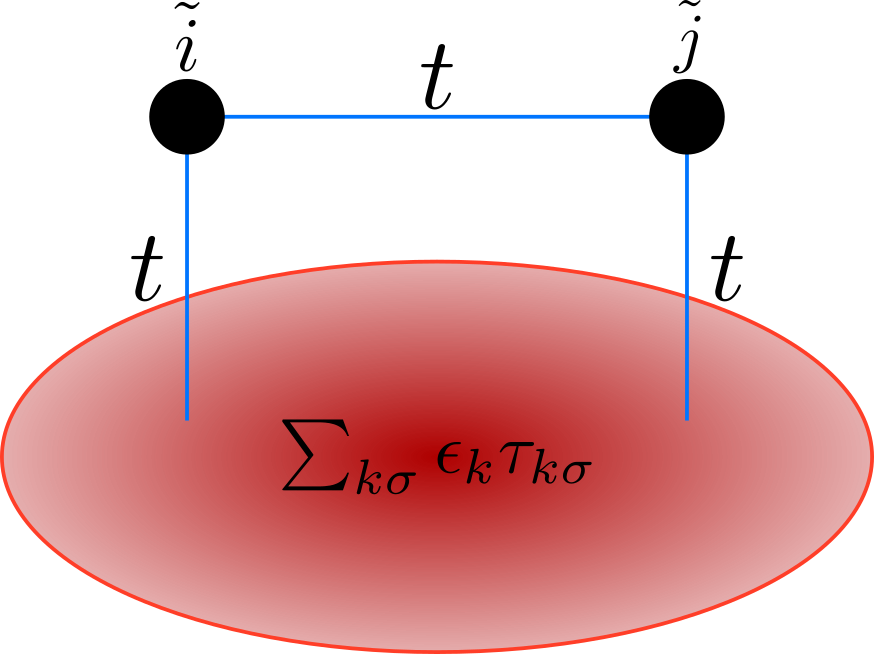
\includegraphics[width=0.2\textwidth]{dimer_dispersion.png}
	\caption{Hubbard dimer with dispersion that connects to both sites}
\end{figure}
\par\noindent
By systematically increasing the number of momentum states in the bath dispersion, we can systematically improve the numerical computation of the ground state wavefunction. From here, we can compute matrix elements of $H^{D}$, and hence the functions $g_0$ and $g_1$. The presence of the bath can be understood as follow. In the absence of a bath, i.e., we have just a Hubbard dimer, an electron can at most hop between the two sites and lead to the wavefunction in eq.~\ref{guess}. However, with a single particle hopping term connecting the dimer to a bath, an electron can also journey between the two sites of the bath via the bath. This leads to entanglement between the dimer's sites and those in the bath; this was clearly ignored in the ground state wavefunction eq.~\ref{guess}. The introduction of the bath dispersion offers the possibility that we can capture a site diagonal spectral function of the three peak form, because we have previously seen such a spectral function in the fixed point of the URG analysis of the SIAM (where the fixed point effective Hamiltonian was an Anderson molecule with dispersion). If this can be found, then a metal-insulator transition of the full Hubbard model can perhaps be captured by studying the spectral functions of the bath-coupled Hubbard dimer.
\item Another improvement can be made by introducing a self-energy $\Sigma (k,\omega)$ into the bath dispersion. This introduces correlation within the bath. The Hamiltonian that we would need to solve would be the same as eq.~\ref{dimer_dispersion}, but with $\epsilon_k$ replaced by $\tilde \epsilon_k \equiv \epsilon_k + \Sigma(k,\omega)$. The self-energy $\Sigma (k,\omega)$ will have to be chosen depending on the phase we want to look at (e.g., metal, insulator etc.). With a $\Sigma$ that is singular near the Fermi surface at $\omega \to 0$, the dispersion will become gapped and the phase will be insulating. In such a situation, there are no low-energy bath excitations within a given energy window proximate to its putative Fermi energy. This will localise the bath electrons, as well as confine all journeys between the two sites of the dimer to only the direct path. This is an indication of the localisation of electrons in the Hubbard model to holon-doublon excitations on nearest neighbour sites. In such a circumstance, eq.~\ref{guess} will be a very good approximation to the actual insulating ground state of the Hubbard model. On the other hand, if we use a self energy that vanishes near the Fermi surface ($\Sigma(\omega) \sim \omega^2$, i.e., a Fermi liquid bath), then we expect to end up in a metallic phase of the Hubbard model. This is simply due to the possibility of holons and doublons now dispersing throughout the lattice, and be concomitant with the presence of a pole in the single-particle Greens function $G(k,\omega)$ of the Hubbard model. Introducing the self energy therefore gives us a larger variety of wavefunctions and features to work with. Further, this appears to be in line with the original proposals offered by Mott and Kohn for the Mott metal insulator transition as the localisation-delocalisation transition of holon-doublon pairs. With regards to the transition itself, the precise form of the bath $\Sigma (k,\omega)$ (or spectral function) remains to be determined.
\end{enumerate}
Once we have chosen a test Hamiltonian whose wavefunction we can calculate, we can use that to obtain the ground state energy of this state. The wavefunction will act as our $\ket{0}$ and the ground state energy will be our $E_\text{GS}$. We can then substitute these into the Lehmann representation form of the Greens function, and calculate the matrix elements $\mathcal{G}_D(\omega)_{\nu \nu^\prime}$ and $\mathcal{G}_D(-\omega)_{\overline{\nu \nu^\prime}}$ for the Hubbard dimer Hamiltonian. Each set will form a $2\times2$ matrix, and we can invert them to obtain $\mathcal{G}_D(\omega)$, and then the matrix elements of this inverted matrix will give all the parameters $g_0$ through $\overline{g_1}$.

\section{Analytic consistency checks}
\subsection{Single-particle Greens function and self energy for the Hubbard dimer}
The simplest test involves choosing $H^H = H^D$ and then calculating the momentum space Greens function at $k=0$, $G(k=0, \uparrow)$, for the Hubbard dimer \(\left(N = 2, w = 1 \right)\). The discrete set of momenta are \(\left\{ \vec k_n \right\} = 0, \frac{\pi}{a}\). For $k=0$, we have
\begin{equation}\begin{aligned}
	\xi_{\vec k = 0} = e^{ikr} = 1
\end{aligned}\end{equation}
Substituting this into eq.~\ref{k_Gf} gives
\begin{equation}\begin{aligned}
	\label{Gk_dim}
	G(k=0,\uparrow) = \sum_n\left[\left(|C^0_{n}|^2 + {C^0_{n}}^* C^1_{n} \right)\frac{1}{g_n} - \left(|\overline C^0_{n}|^2 + {\overline C^0_{n}}^* \overline C^1_{n}\right)\frac{1}{\overline{g_n}}\right]
\end{aligned}\end{equation}
The expansion in terms of the exact eigenstates takes the form:
\begin{equation}\begin{aligned}
	c^\dagger_{0 \uparrow}\ket{\tilde \Phi_0} = x\ket{3+ \uparrow} + y\ket{3- \uparrow}, && c^\dagger_{1 \uparrow}\ket{\tilde \Phi_0} = x\ket{3+ \uparrow} - y\ket{3- \uparrow}\\
	c_{0 \uparrow}\ket{\tilde \Phi_0} = y\ket{1+ \downarrow} + x\ket{1- \downarrow}, && c_{1 \uparrow}\ket{\tilde \Phi_0} = y\ket{1+ \downarrow} - x\ket{1- \downarrow}\\
\end{aligned}\end{equation}
where $\ket{(3,1)\pm (\uparrow, \downarrow)}$ are the $N=(3,1), S^z = (+\frac{1}{2}, -\frac{1}{2})$ eigenstates of even $(+)$ and odd \((-)\) parity:
\begin{equation}\begin{aligned}
	H^D\ket{3\pm \uparrow} = \pm t \ket{3\pm \uparrow}\\
	H^D\ket{1\pm \downarrow} = \mp t \ket{1\pm \downarrow}\\
\end{aligned}\end{equation}
and \(x = \frac{a_2 - a_1}{2}, y = \frac{a_2 + a_1}{2}\). The orthogonal basis is therefore
\begin{equation}\begin{aligned}
	\left\{ \ket{n} \right\} = \ket{3+ \uparrow}, \ket{3- \uparrow}\\
	\left\{ \ket{\overline n} \right\} = \ket{1+ \downarrow}, \ket{1- \downarrow}
\end{aligned}\end{equation}
The coefficients can thus be determined:
\begin{gather*}
	C^0_\pm = \braket{3\pm \uparrow|c^\dagger_{0 \uparrow} |\tilde \Phi_0} = x, y\\
	C^1_\pm = \braket{3\pm \uparrow|c^\dagger_{1 \uparrow} |\tilde \Phi_0} = x, -y\\
	\overline C^0_\pm = \braket{1 \pm \downarrow|c_{0 \uparrow} |\tilde \Phi_0} = y, x\\
	\overline C^1_\pm = \braket{1 \pm \downarrow|c_{1 \uparrow} |\tilde \Phi_0} = y, -x\\
	g_\pm = \bra{3 \pm \uparrow}\left( \omega + E_{GS} - H^D\right) \ket{3 \pm \uparrow} = \omega + E_{GS} \mp t\\
	\overline{g_\pm} = \bra{1 \pm \downarrow}\left(-\omega + E_{GS} - H^D\right) \ket{1 \pm \downarrow} = -\omega + E_{GS} \pm t\\
\end{gather*}
We can see that $|C^0_-|^2 + {C^0_-}^* C^1_- = y^2 - y^2 = 0$ and $|\overline C^0_-|^2 + {\overline C^0_-}^* \overline C^1_- = x^2 - x^2 = 0$. So we do not need to consider those terms. With this preparation, we can now calculate the Greens function:
\begin{equation}\begin{aligned}
	G(k=0, \omega) = \left(|C^0_{+}|^2 + {C^0_{+}}^* C^1_{+} \right)\frac{1}{g_+} - \left(|\overline C^0_{+}|^2 + {C^0_{+}}^* \overline C^1_{+}\right)\frac{1}{\overline{g_+}} = \frac{2x^2}{\omega + E_{GS} - t} - \frac{2y^2}{-\omega + E_{GS} + t}
\end{aligned}\end{equation}
The final step is to recognize that $2x^2 = \frac{a_1^2 + a_2^2 -2a_1a_2}{2} = \frac{1}{2} - \frac{2t}{\Delta}$, $2y^2 = \frac{a_1^2 + a_2^2 + 2a_1a_2}{2} = \frac{1}{2} + \frac{2t}{\Delta}$ and $E_{GS} = -\frac{\Delta}{2}$. Then,
\begin{equation}\begin{aligned}
	G(k=0, \omega) = \frac{\frac{1}{2} - \frac{2t}{\Delta}}{\omega - \frac{\Delta}{2} - t} - \frac{\frac{1}{2} + \frac{2t}{\Delta}}{-\omega - \frac{\Delta}{2} + t} = \frac{\frac{1}{2} - \frac{2t}{\Delta}}{\omega - \frac{\Delta}{2} - t} + \frac{\frac{1}{2} + \frac{2t}{\Delta}}{\omega + \frac{\Delta}{2} - t}
\end{aligned}\end{equation}



% We will now calculate the matrix elements $g_0$ and $g_1$ from the Hubbard dimer Hamiltonian. Those two parameters are defined as
% \begin{equation}\begin{aligned}
% 	g_0 \equiv \frac{2}{N}\bra{\text{GS}}c_{0\uparrow}\left(\omega + E_\text{GS} - H^D\right)c^\dagger_{0\uparrow}\ket{\text{GS}}\\
% 	g_1 \equiv \frac{2}{N}\bra{\text{GS}}c_{0\uparrow}\left(\omega + E_\text{GS} - H^D\right)c^\dagger_{1\uparrow}\ket{\text{GS}}\\
% \end{aligned}\end{equation}
% As a shorthand notation, we will use $\ket{0 \sigma} \equiv c^\dagger_{0\uparrow}\ket{\text{GS}}$. The matrix whose elements we want to calculate, $\omega + E_\text{GS} - H^D$, can be written as a diagonal matrix in the basis formed by the eigenstates in $N=3, S^z= \frac{1}{2}$ as defined in table \ref{hubb_dim_spectrum}:
% \begin{equation}\begin{aligned}
% 	\ket{\pm} = \frac{1}{\sqrt 2}\left(\ket{\uparrow, 2} \pm \ket{2, \uparrow}\right), && H^D \ket{\pm} = E_\pm \ket{\pm}
% \end{aligned}\end{equation}
% In the basis of $\ket{\pm}$, we can write
% \begin{equation}\begin{aligned}
% 	\omega + E_\text{GS} - H^D &= \begin{pmatrix} \omega + E_\text{GS} - E_+ & 0 \\ 0 & \omega + E_\text{GS} - E_- \end{pmatrix}\\
% 				   &= \left(\omega + E_\text{GS} - E_+\right) \ket{+}\bra{+} + \left(\omega + E_\text{GS} - E_-\right) \ket{-}\bra{-}
% \end{aligned}\end{equation}
% The excited state $c^\dagger_{0\uparrow}\ket{\text{GS}}$ can actually be written in terms of the $N=3$, $S^z = + \frac{1}{2}$ eigenstates. As shown in the appendix, we can write
% \begin{equation}\begin{aligned}
% 	\ket{0 \uparrow} \equiv c^\dagger_{0\uparrow}\ket{\text{GS}} =x\ket{+} + y\ket{-}, && \ket{1 \uparrow} \equiv c^\dagger_{1\uparrow}\ket{\text{GS}} = x\ket{+} - y\ket{-}
% \end{aligned}\end{equation}
% with $x = \frac{a_2 - a_1}{2}, y=\frac{a_2 + a_1}{2}$. We can therefore express $\ket{\pm}$ in terms $\ket{0,1\uparrow}$:
% \begin{equation}\begin{aligned}
% 	\ket{+} = \frac{1}{2x}\left(\ket{0 \uparrow} + \ket{1 \uparrow}\right), && \ket{-} = \frac{1}{2y}\left(\ket{0 \uparrow} - \ket{1 \uparrow}\right)
% \end{aligned}\end{equation}
% Substituting these into the operator form of $\omega + E_\text{GS} - H^D$ gives
% \begin{equation}\begin{aligned}
% 	\omega + E_\text{GS} - H^D =& \frac{1}{4x^2}\left(\omega + E_\text{GS} - E_+\right) \left(\ket{0 \uparrow} + \ket{1 \uparrow}\right)\left(\bra{0 \uparrow} + \bra{1 \uparrow}\right) \\
% 				   &+ \frac{1}{4y^2}\left(\omega + E_\text{GS} - E_-\right) \left(\ket{0 \uparrow} - \ket{1 \uparrow}\right)\left(\bra{0 \uparrow} - \bra{1 \uparrow}\right)\\
% =& \begin{pmatrix}\left(\frac{1}{4x^2} + \frac{1}{4y^2}\right) \left(\omega + E_\text{GS}\right) - \frac{1}{4x^2}E_+ - \frac{1}{4y^2}E_- & \left(\frac{1}{4x^2} - \frac{1}{4y^2}\right) \left(\omega + E_\text{GS}\right) - \frac{1}{4x^2}E_+ + \frac{1}{4y^2}E_- \\ \left(\frac{1}{4x^2} - \frac{1}{4y^2}\right) \left(\omega + E_\text{GS}\right) - \frac{1}{4x^2}E_+ + \frac{1}{4y^2}E_- & \left(\frac{1}{4x^2} + \frac{1}{4y^2}\right) \left(\omega + E_\text{GS}\right) - \frac{1}{4x^2}E_+ - \frac{1}{4y^2}E_-\end{pmatrix} 
% \end{aligned}\end{equation}
% Now we will Fourier transform to the diagonal momentum space: $\ket{0 \sigma} = \frac{1}{\sqrt 2}\left(\ket{{k_0} \sigma} + \ket{k_\pi \sigma} \right), \ket{1 \sigma} = \frac{1}{\sqrt 2}\left(\ket{{k_0} \sigma} - \ket{k_\pi \sigma} \right)$.
% \begin{equation}\begin{aligned}
% 	\left(\ket{0 \uparrow} + \ket{1 \uparrow}\right)\left(\bra{0 \uparrow} + \bra{1 \uparrow}\right) = 2\ket{k_0 \uparrow}\bra{k_0 \uparrow}\\
% 	\left(\ket{0 \uparrow} - \ket{1 \uparrow}\right)\left(\bra{0 \uparrow} - \bra{1 \uparrow}\right) = 2\ket{k_\pi \uparrow}\bra{k_\pi \uparrow}\\
% \end{aligned}\end{equation}
% This transformation can be substituted in the operator expansion:
% \begin{equation}\begin{aligned}
% 	\omega + E_\text{GS} - H^D =& \frac{1}{2x^2}\left(\omega + E_\text{GS} - E_+\right) \ket{k_0 \uparrow}\bra{k_0 \uparrow} + \frac{1}{2y^2}\left(\omega + E_\text{GS} - E_-\right) \ket{k_\pi \uparrow}\bra{k_\pi \uparrow}\\
% \end{aligned}\end{equation}
% This can be easily inverted:
% \begin{equation}\begin{aligned}
% 	\frac{1}{\omega + E_\text{GS} - H^D} =& \frac{2x^2}{\omega + E_\text{GS} - E_+}\ket{k_0 \uparrow}\bra{k_0 \uparrow} + \frac{2y^2}{\omega + E_\text{GS} - E_-} \ket{k_\pi \uparrow}\bra{k_\pi \uparrow}\\
% \end{aligned}\end{equation}
% Since this is already in the momentum space basis, we can write
% \begin{equation}\begin{aligned}
% 	\left(\frac{1}{\omega + E_\text{GS} - H^D}\right)_{k_0 k_0} = \frac{2x^2}{\omega + E_\text{GS} - E_+}\ket{k_0 \uparrow}
% \end{aligned}\end{equation}
% Performing a similar calculation for the hole excitations will give
% \begin{equation}\begin{aligned}
% 	\frac{1}{-\omega + E_\text{GS} - H^D} =& \frac{2y^2}{-\omega + E_\text{GS} - \overline{E_+}}\ket{\overline{k_0 \uparrow}}\bra{\overline{k_0 \uparrow}} + \frac{2x^2}{-\omega + E_\text{GS} - \overline{E_-}} \ket{\overline{k_\pi \uparrow}}\bra{\overline{k_\pi \uparrow}}\\
% \end{aligned}\end{equation}
% where $\ket{\overline{\nu}} \equiv c_\nu \ket{\text{GS}}$ and $\overline{E_\pm}$ are the eigenenergies of the $N=1, S^z = \frac{1}{2}$ sector eigenstates. From the spectrum, we know that $E_\pm = -\overline{E_\pm}$.\\\\
% Combining these two, we can obtain the $k=0$ Greens function of the Hubbard dimer:
% \begin{equation}\begin{aligned}
% 	G(k=0, \uparrow) &= \left(\frac{1}{\omega + E_\text{GS} - H^D}\right)_{k_0 k_0} - \left(\frac{1}{-\omega + E_\text{GS} - H^D}\right)_{\overline{k_0 k_0}}\\
% 			 &= \frac{2x^2}{\omega + E_\text{GS} - E_+} - \frac{2y^2}{-\omega + E_\text{GS} - \overline{E_+}}\\
% 			 &= \frac{2x^2}{\omega + E_\text{GS} - E_+} + \frac{2y^2}{\omega - E_\text{GS} - E_+}\\
% \end{aligned}\end{equation}
% From the definitions of $x$ and $y$, we get $2x^2 = \frac{a_1^2 + a_2^2 - 2a_1 a_2}{2} = \frac{1}{2} - \frac{2t}{\Delta}$ and $2y^2 = \frac{1}{2} + \frac{2t}{\Delta}$. Also, the ground state energy is $E_\text{GS} = -\frac{\Delta}{2}$ and the excited energy $E_+$ is $t$. Substituting these gives
% \begin{equation}\begin{aligned}
% 	G(k=0, \uparrow) &= \frac{\frac{1}{2} - \frac{2t}{\Delta}}{\omega - \frac{\Delta}{2} - t} + \frac{\frac{1}{2} + \frac{2t}{\Delta}}{\omega + \frac{\Delta}{2} - t}\\
% \end{aligned}\end{equation}

% from the Greens function matrices of the Hubbard dimer. From the spectral representation of the Greens function matrix elements in eq.~\ref{G_mat_spec}, we obtain
% \begin{equation}\begin{aligned}
% 	\left(\mathcal{G}_D\right)_{\nu \nu^\prime} = \begin{pmatrix} x_- + y_- && x_- - y_- \\ x_- - y_- && x_- + y_- \end{pmatrix}
% \end{aligned}\end{equation}
% where
% \begin{equation}\begin{aligned}
% 	x_\pm \equiv \left( \frac{1}{4} \pm \frac{t}{\Delta} \right) \frac{1}{\mp\omega - \frac{\Delta}{2} \pm t}, && y_\pm \equiv \left( \frac{1}{4} \mp \frac{t}{\Delta} \right) \frac{1}{\mp\omega - \frac{\Delta}{2} \mp t}
% \end{aligned}\end{equation}
% The matrix is easily inverted:
% \begin{equation}\begin{aligned}
% 	\left(\mathcal{G}_D^{-1}\right)_{\nu \nu^\prime}(\omega) = \frac{1}{4}\begin{pmatrix}  \frac{1}{x_-} + \frac{1}{y_-} &&  \frac{1}{x_-} - \frac{1}{y_-} \\  \frac{1}{x_-} - \frac{1}{y_-} &&  \frac{1}{x_-} + \frac{1}{y_-} \end{pmatrix}
% \end{aligned}\end{equation}
% $g_0$ and $g_1$ can now be read off:
% \begin{equation}\begin{aligned}
% 	g_0 = \frac{2}{N}\left(\mathcal{G}_D^{-1}\right)_{00} = \frac{1}{4}\left( \frac{1}{x_-} + \frac{1}{y_-}\right), && g_1 = \frac{2}{N}\left(\mathcal{G}_D^{-1}\right)_{01} = \frac{1}{4}\left( \frac{1}{x_-} - \frac{1}{y_-}\right)
% \end{aligned}\end{equation}
% Similarly, we obtain the other matrix:
% \begin{equation}\begin{aligned}
% 	\left(\mathcal{G}_D\right)_{\overline{\nu \nu^\prime}}(-\omega) = \begin{pmatrix} x_+ + y_+ && x_+ - y_+ \\ x_+ - y_+ && x_+ + y_+ \end{pmatrix}
% \end{aligned}\end{equation}
% which gives
% \begin{equation}\begin{aligned}
% 	\overline{g_0} = \frac{2}{N}\left(\mathcal{G}_D^{-1}\right)_{00} = \frac{1}{4}\left( \frac{1}{x_+} + \frac{1}{y_+}\right), && \overline{g_1} = \frac{2}{N}\left(\mathcal{G}_D^{-1}\right)_{01} = \frac{1}{4}\left( \frac{1}{x_+} - \frac{1}{y_+}\right)
% \end{aligned}\end{equation}
% Substituting these values of $g_0, g_1, \overline{g_0}$ and $\overline{g_1}$ in eq.~\ref{Gk_dim} gives the same expression as that obtained in eq.~\ref{Gk0}.

%To verify this result, we just need to show the momentum space Greens function of the Hubbard dimer calculated from the exact eigenstates (as shown in the appendix) also takes the same form. Using the Fourier transform, we can write
%\begin{equation}\begin{aligned}
%	G(k=0, \sigma) = G(r=0, \sigma) + G(r=a, \sigma)
%\end{aligned}\end{equation}
%The terms on the RHS are the real space local and nearest-neighbour Greens functions of the Hubbard dimer.
%Therefore, the Greens function at $\vec r=0$ for the Hubbard dimer can be expressed as
%\begin{equation}\begin{aligned}
%	G_H(\vec r = 0, \omega) = \frac{1}{2}\left[\frac{1}{g_0 + g_1} + \frac{1}{g_0 - g_1}\right]  = \frac{g_0}{g_0^2 - g_1^2}
%\end{aligned}\end{equation}
%For the Hubbard dimer, we substitute $N=2, w=1$ into the expressions for $g_{0}$ and $g_{1}$ to obtain
%\begin{equation}\begin{aligned}
%	&g_0 = \frac{1}{\text{Det }G_D}\left( G_D \right)_{00}, &g_1 = -\frac{1}{\text{Det }G_D}\left( G_D \right)_{01}
%\end{aligned}\end{equation}
%The Greens function at the zeroth site then becomes
%\begin{equation}\begin{aligned}
%	G_H(\vec r = 0, \omega) = \text{Det }G_D\frac{\left(G_D\right)_{00}}{\left(G_D\right)_{00}^2 - \left(G_D\right)_{01}^2} = \text{Det }G_D\frac{\left(G_D\right)_{00}}{\text{Det }G_D} = \left(G_D\right)_{00}
%\end{aligned}\end{equation}
%This is the expected result. Because the full Hubbard model in this case was simply the Hubbard dimer, \(G_H(\vec r = 0, \omega)\) should just be \(\left(G_D\right)_{00}\). Although this is a trivial example (we matched the Hubbard dimer with another Hubbard dimer), this atleast tells us that this algorithm for calculating the real space local Greens function from the inverse Greens function matrix elements is sensible.

\subsection{On the Bethe lattice}
Another test involves considering the case of infinite number of nearest neighbours $w\to\infty$ (the coordination number, and effectively the dimensionality). Here, as has been argued in the DMFT literature, the correct scaling of the $t^{H}$ hopping parameter is $t^{H}\to t^{H}/\sqrt{w}$ such that the kinetic energy of the associated tight-binding lattice model is finite. This allows for the competition between the kinetic and potential terms of the Hamiltonian to drive a metal-insulator transition in the limit of $w\to\infty$ as well. Further, it has been argued in the DMFT literature that the Greens function matrix of the Hubbard model on the Bethe lattice with $w\to\infty$ becomes purely local (i.e., it has vanishing inter-site matrix elements). We can also see this from eqs.\eqref{G_mat_nn}- the nearest-neighbour inverse Greens function vanishes in the limit of $w \to \infty$:
\begin{equation}\begin{aligned}
	\left(\mathcal{G}_{H}(\omega)\right)_{ij}^\sigma = \frac{2}{Nw}\sum_{n} {\overline C^0_{n}}^* \overline C^1_{n} \frac{1}{\overline{g_n}} \implies \lim_{w \to \infty}\left(\mathcal{G}_{H}(\omega)\right)_{ij}^\sigma \to 0
\end{aligned}\end{equation}
There we used the fact since at half-filling on an $SU(2)$ symmetric mode, we expect $\left<\hat n_{i \uparrow} \right> = \frac{1}{2}$, the orthonormal expansion of $c^\dagger_{i \sigma}\ket{\tilde \Phi_0} = \sum_n C^i_n \ket{n}$ to be constrained to $\sum_n |C_n^i|^2 = \frac{1}{2}$, such that the only term that scales with $w$ is $w$ itself. This result then implies that $G^{H}$ matrix has no $k$ dependence. 
\\\\
In this limit, the self-energy also simplifies:
\begin{equation}\begin{aligned}
	\lim_{w \to \infty}\Sigma_H(\vec k,\omega) &= \omega +t^{H}\xi_{\vec k} - \frac{N}{2}\left\{\sum_n \lim_{w \to \infty}\left[\left(|C^0_{n}|^2 + \frac{\xi_{\vec{k}}}{w}{C^0_{n}}^* C^1_{n} \frac{1}{g_n}\right)\frac{1}{g_n} - \left(|\overline C^0_{n}|^2 + \frac{\xi_{\vec{k}}}{w}{\overline C^0_{n}}^* \overline C^1_{n}\right)\frac{1}{\overline{g_n}}\right]\right\}^{-1} \\
						   &=\omega +t^{H}\xi_{\vec k} - \frac{N}{2}\frac{1}{\sum_n \left[ \frac{|C^0_{n}|^2}{g_n} - \frac{|\overline C^0_{n}|^2}{\overline{g_n}}\right]}
\end{aligned}\end{equation}
We can now see that even in the limit of $w\to\infty$, the competition between ${g}_{0}$ (the on-site repulsion) and the hopping related kinetic energy ($t^{H}\xi_{\vec{k}}$) can lead to a metal-insulator transition.

\section{Future goals}
\begin{enumerate}
\item Obtain the metal insulator transition of the 2D Hubbard model on the square lattice from our formalism. Compare with what is obtained from DMFT and its improvements. Also, determine the nature of the bath $\Sigma (k,\omega)$ for the transition point.

\item Once the zero temperature Mott metal-insulator transition is observed, we will investigate its nature.

\item While we have provided expressions for the single particle Greens functions of the $N$-site Hubbard model from their equivalent single particle Greens functions of the Hubbard dimer, we expect that eq.\eqref{green_eq_final} holds quite generally for the two-particle Greens function sector as well. We will provide these expressions at a later point in time. More specifically, we will calculate the Greens functions for holon-doublon and spinon-spinon excitations as they are likely to contain more information regarding the ground state.

\item It is also important to benchmark the ground state energy and double occupancy obtained from this method against the ground state wavefunction obtained from exact diagonalisation of small lattices and finite size scaling.

\item It should also prove instructive to investigate the nature of many-particle entanglement in the ground state wavefunction of various phases, and  look for signs of a quantum liquid.

\item Once we have a handle on the zero temperature features, we intend to compute Greens functions at non zero temperatures.

\item This method can also be extended to various other models of strong correlation:
	\begin{enumerate}
		\item Heisenberg model, by starting from a Kondo model effective Hamiltonian
		\item Periodic Anderson model, by starting from a SIAM with a dispersive bath
		\item Periodic Kondo model, by starting from a Kondo model with a dispersive bath
		\item Hubbard-Heisenberg model, by starting from a generalized Anderson molecule (Anderson molecule with two-particle spin and charge interactions between the two sites)
	\end{enumerate}
\end{enumerate}

\newpage
\section*{Appendix: Spectra of Hubbard dimer}
Here we document the spectrum of the Hamiltonian in eqs.~\ref{hubb_dimer}.
\begin{center}
	\begin{tabular}{|c|c|c|}
	\hline
	eigenstate & symbol & eigenvalue \\
	\hline
	$\ket{0,0}$ & $\ket{0}$ & \( \frac{U^H}{2}\)\\
	$ \frac{1}{\sqrt 2}\left(\ket{\sigma,0} \pm \ket{0,\sigma}\right)$ & $\ket{0\sigma_\pm}$ & \(\mp t^H\)\\
	$\ket{\sigma,\sigma}$ & $\ket{\sigma\sigma}$ & \( -\frac{U^H}{2}\)\\
	$ \frac{1}{\sqrt 2}\left(\ket{\uparrow,\downarrow} + \ket{\downarrow,\uparrow}\right)$ & $\ket{ST}$ & \( -\frac{U^H}{2}\)\\
	$ \frac{1}{\sqrt 2}\left(\ket{2,0} - \ket{0,2}\right)$ & $\ket{CS}$ & \( \frac{U^H}{2}\)\\
	$a_1(U^H, t^H) \frac{1}{\sqrt 2}\left(\ket{\uparrow,\downarrow} - \ket{\downarrow,\uparrow}\right) + a_2(U^H, t^H)\frac{1}{\sqrt 2}\left(\ket{2,0} + \ket{0,2}\right)$ & $\ket{-}$ & \(-\frac{1}{2}\Delta(U^H, t^H)\)\\
	$-a_2(U^H, t^H) \frac{1}{\sqrt 2}\left(\ket{\uparrow,\downarrow} - \ket{\downarrow,\uparrow}\right) + a_1(U^H, t^H)\frac{1}{\sqrt 2}\left(\ket{2,0} + \ket{0,2}\right)$ & $\ket{+}$ & \(\frac{1}{2}\Delta(U^H, t^H)\)\\
	$ \frac{1}{\sqrt 2}\left(\ket{\sigma,2} \pm \ket{2,\sigma}\right)$ & $\ket{2\sigma_\pm}$ & \(\pm t^H\)\\
	$\ket{2,2}$ & $\ket{4}$ & \( \frac{U^H}{2}\)\\
\hline
	\end{tabular}
	\captionof{table}{Spectrum of Hubbard dimer at half-filling}
	\label{hubb_dim_spectrum}
%	\begin{tabular}{|c|c|c|}
%	\hline
%	eigenstate & symbol & eigenvalue\\
%	\hline
%	\(\ket{0,0}\) & \(\ket{0}\) & \(\frac{U^A}{4}\)\\
%	\(a_1\left(U^A, t^A\right)\ket{\sigma,0} + a_2\left(U^A, t^A\right)\ket{0, \sigma}\) & \(\ket{0\sigma_-}\) & \(-\frac{1}{4}\Delta(U^A, t^A)\)\\
%	\(-a_2\left(U^A, t^A\right)\ket{\sigma,0} + a_1\left(U^A, t^A\right)\ket{0, \sigma}\) & \(\ket{0\sigma_+}\) & \(\frac{1}{4}\Delta(U^A, t^A)\)\\
%	\(\ket{\sigma,\sigma}\) & \(\ket{\sigma\sigma}\) & \(-\frac{U^A}{4}\)\\
%	\(\frac{1}{\sqrt 2}\left(\ket{\uparrow, \downarrow} + \ket{\downarrow, \uparrow}\right)\) & \(\ket{ST}\) & \(-\frac{U^A}{4}\)\\
%	\(\frac{1}{\sqrt 2}\left(\ket{2, 0} - \ket{0, 2}\right)\) & \(\ket{CS}\) & \(\frac{U^A}{4}\)\\
%	$a_1( \frac{1}{2}U^A, t^A) \frac{1}{\sqrt 2}\left(\ket{\uparrow,\downarrow} - \ket{\downarrow,\uparrow}\right) + a_2( \frac{1}{2}U^A, t^A)\frac{1}{\sqrt 2}\left(\ket{2,0} + \ket{0,2}\right)$ & $\ket{-}$ & \(-\frac{1}{2}\Delta( \frac{1}{2}U^A, t^A)\)\\
%	$-a_2(\frac{1}{2}U^A, t^A) \frac{1}{\sqrt 2}\left(\ket{\uparrow,\downarrow} - \ket{\downarrow,\uparrow}\right) + a_1(\frac{1}{2}U^A, t^A)\frac{1}{\sqrt 2}\left(\ket{2,0} + \ket{0,2}\right)$ & $\ket{+}$ & \(\frac{1}{2}\Delta(\frac{1}{2}U^A, t^A)\)\\
%	\(a_1\left(U^A, t^A\right)\ket{\sigma,2} - a_2\left(U^A, t^A\right)\ket{2, \sigma}\) & \(\ket{2\sigma_-}\) & \(-\frac{1}{4}\Delta(U^A, t^A)\)\\
%	\(a_2\left(U^A, t^A\right)\ket{\sigma,2} + a_1\left(U^A, t^A\right)\ket{2, \sigma}\) & \(\ket{2\sigma_+}\) & \(\frac{1}{4}\Delta(U^A, t^A)\)\\
%	\(\ket{2,2}\) & \(\ket{4}\) & \(\frac{U^A}{4}\)\\
%	\hline
%	\end{tabular}
%	\captionof{table}{Spectrum of Anderson molecule at particle-hole symmetry}
\end{center}
\section*{Appendix: Local Greens function for the Hubbard dimer}
From the spectral representation, we have the following expression for the local Greens function for the Hubbard dimer at site $0$:
\begin{equation}\begin{aligned}
	G_{D,00}^\sigma(\omega) = \frac{1}{Z}\sum_{m,n}||\bra{m}c_{i\sigma}\ket{n}||^2\left( e^{-\beta E_m} + e^{-\beta E_n}\right)\frac{1}{\omega + E_m - E_n}
\end{aligned}\end{equation}
$m,n$ sum over the exact eigenstates. $E_m, E_n$ are the corresponding energies. We are interested in teh $T \to 0$ Greens function. In that limit, all exponentials except that for the ground state $E_{gs}$ will die out. The exponential inside the summation will then cancel the exponential in the partition function.
\begin{equation}\begin{aligned}
	G_{D,00}^\sigma(\omega, T \to 0) &= \sum_{n}\left[||\bra{GS}c_{i\sigma}\ket{n}||^2\frac{1}{\omega + E_{GS} - E_n} + ||\bra{n}c_{i\sigma}\ket{GS}||^2\frac{1}{\omega + E_n - E_{GS}}\right]\\
					&= \sum_{n}\left[||\bra{n}c^\dagger_{i\sigma}\ket{GS}||^2\frac{1}{\omega + E_{GS} - E_n} + ||\bra{n}c_{i\sigma}\ket{GS}||^2\frac{1}{\omega + E_n - E_{GS}}\right]\\
\end{aligned}\end{equation}

The ground state $\ket{GS}$ is just the state $\ket{-}$ in the table \ref{hubb_dim_spectrum}. We will choose to look at $\sigma = \uparrow`$. Then,
\begin{equation}\begin{aligned}
	c_{1\uparrow}\ket{-} &= \frac{a_1}{\sqrt 2}\ket{0, \downarrow} + \frac{a_2}{\sqrt 2}\ket{\downarrow,0}\\
	c^\dagger_{1\uparrow}\ket{-} &= -\frac{a_1}{\sqrt 2}\ket{2, \uparrow} + \frac{a_2}{\sqrt 2}\ket{\uparrow,2}\\
\end{aligned}\end{equation}
The set of states $\ket{n}$ that give non-zero inner product $\ket{GS}$ are therefore
\begin{equation}\begin{aligned}
	\left\{ \ket{n} \right\} &= \ket{0\downarrow_\pm}\\
	||\bra{n}c_{\uparrow\sigma}\ket{GS}||^2 &= \frac{1}{4}\left(a_2 \pm a_1 \right)^2 = \frac{1}{4}\left(1 \pm 2a_1a_2\right)\\
	\left\{ E_n \right\} &= \mp t
\end{aligned}\end{equation}
for the second inner product, and
\begin{equation}\begin{aligned}
	\left\{\ket{n}\right\} &= \ket{2\uparrow_\pm}\\
	||\bra{n}c^\dagger_{\uparrow\sigma}\ket{GS}||^2 &= \frac{1}{4}\left( a_2 \mp a_1 \right)^2 = \frac{1}{4}\left(1 \mp 2a_1a_2\right)\\
	\left\{ E_n \right\} &= \pm t
\end{aligned}\end{equation}
for the first. The Greens function is therefore
\begin{equation}\begin{aligned}
	\label{dimer_local_G}
	G_{D,00}^\uparrow(\omega, T \to 0) &= \left( \frac{1}{2} + \frac{2t}{\Delta} \right) \frac{\omega}{\omega^2 - \left(t - \frac{\Delta}{2}\right) ^2} + \left( \frac{1}{2} - \frac{2t}{\Delta} \right) \frac{\omega}{\omega^2 - \left(t + \frac{\Delta}{2}\right) ^2} = G_{D,00}^\downarrow(\omega, T \to 0)~.
\end{aligned}\end{equation}
In the atomic limit $(t=0)$, the Greens function simplifies to
\begin{equation}\begin{aligned}
	G_{D,00}^\uparrow(\omega, T \to 0) \bigg\vert_\text{atomic} = \frac{\omega}{\omega^2 - \frac{1}{4}U^2}
\end{aligned}\end{equation}
In the atomic limit, the singly-occupied state has zero energy:
\begin{equation}\begin{aligned}
	E_1(t=0) = \bra{1,0}\left(U \tau_{0 \uparrow}\tau_{0 \downarrow} + U \tau_{1 \uparrow}\tau_{1 \downarrow}\right) \ket{1,0} = 0
\end{aligned}\end{equation}
We can write the atomic limit Greens function in terms of this energy and the self energy:
\begin{equation}\begin{aligned}
	G_{D,00}^\uparrow(\omega, T \to 0) \bigg\vert_\text{atomic} = \frac{1}{\omega - E_1(t=0) - \Sigma(t=0)} = \frac{1}{\omega - 0 -\frac{U^2}{4\omega}}
\end{aligned}\end{equation}
The self energy in the atomic limit can be read off as 
\begin{equation}\begin{aligned}
	\label{dimer_selfenergy}
\Sigma(t=0) = \frac{U^2}{4\omega}
\end{aligned}\end{equation}
The site local spectral function can also be calculated from the local Greens function:
\begin{eqnarray}
A(0\uparrow, \omega) &=& - \frac{1}{\pi}\text{Im }G_{D,00}^\uparrow(\omega)\nonumber\\
			     &=& \left( \frac{1}{4} - \frac{t}{\Delta} \right)\left[\delta(\omega - \frac{1}{2}\Delta - t) + \delta(\omega + \frac{1}{2}\Delta + t)\right]\nonumber\\ 
			     &&+ \left( \frac{1}{4} + \frac{t}{\Delta} \right) \left[\delta(\omega - \frac{1}{2}\Delta + t) + \delta(\omega + \frac{1}{2}\Delta - t)\right]\\ 
			     &=& A(0\downarrow, \omega)~.\nonumber
\end{eqnarray}
Finally, the inter-site Greens function for the Hubbard dimer is given by
\begin{equation}
\label{dimer_intersite_G}
G_{D,01}^\uparrow(\omega, T \to 0) = \left( \frac{1}{2} + \frac{2t}{\Delta} \right) \frac{t - \frac{\Delta}{2}}{\omega^2 - \left(t - \frac{\Delta}{2}\right)^2} + \left( \frac{1}{2} - \frac{2t}{\Delta} \right) \frac{t + \frac{\Delta}{2}}{\omega^2 - \left(t + \frac{\Delta}{2}\right)^2} = G_{D,01}^\downarrow(\omega, T \to 0)~.
\end{equation}
% Once we have calculated the diagonal and off-diagonal matrix elements of the Greens function, we can compute the parameters $g_0$ and $g_1$:
% \begin{equation}\begin{aligned}
%		 g_0 \equiv\frac{2}{N} (G^{-1}_{D})_{00} = \frac{2}{N} \frac{1}{\text{Det }G_D}\left(G_D\right)_{00}, g_1 \equiv\frac{2}{Nw} (G^{-1}_{D})_{00} = -\frac{2}{Nw}\frac{1}{\text{Det }G_D}\left(G_D\right)_{01} 
% \end{aligned}\end{equation}
Using the diagonal and off-diagonal real space Greens functions, we can now compute the momentum-space Greens functions. The two momentum states are $ka = 0, \pi$. By Fourier transforming, these two Greens functions can be written as
\begin{equation}\begin{aligned}
	\label{Gk0}
	G(k=0, \sigma) = \sum_r e^{ikr} G(r, \sigma) = G(r=0, \sigma) + G(r=a, \sigma) = \frac{1/2 + 2t/\Delta}{\omega -t + \Delta/2} + \frac{1/2 - 2t/\Delta}{\omega - t - \Delta/2}\\
	G(k=\pi, \sigma) = \sum_r e^{ikr} G(r, \sigma) = G(r=0, \sigma) - G(r=a, \sigma) = \frac{1/2 + 2t/\Delta}{\omega + t - \Delta/2} + \frac{1/2 - 2t/\Delta}{\omega + t + \Delta/2}\\
\end{aligned}\end{equation}

\section*{Appendix; Contributions of various excitations to the site local spectral function}
The site local spectral function is
\begin{equation}\begin{aligned}
	A(0\uparrow, \omega) = \left( \frac{1}{4} - \frac{t}{\Delta} \right)\left[\delta(\omega - \frac{\Delta}{2} - t) + \delta(\omega + \frac{\Delta}{2} + t)\right]\nonumber + \left( \frac{1}{4} + \frac{t}{\Delta} \right) \left[\delta(\omega - \frac{\Delta}{2} + t) + \delta(\omega + \frac{\Delta}{2} - t)\right]
\end{aligned}\end{equation}
If the eigenstates of the $N=1, S^z = - \frac{1}{2}$ sector are $\ket{1 \pm \downarrow}$ and those of $N=3, S^z = \frac{1}{2}$ sector are $\ket{3 \pm \uparrow}$, this spectral function originates from the expression:
\begin{equation}\begin{aligned}
	A(0\uparrow, \omega) =& \braket{1 \downarrow_- | c_{0 \uparrow} | \text{GS}} \delta\left(\omega + \frac{\Delta}{2} + t\right) + \braket{2 \uparrow_+ | c^\dagger_{0 \uparrow} | \text{GS}}\delta\left(\omega - \frac{\Delta}{2} - t\right) \\
			      &+ \braket{1 \downarrow_+ | c_{0 \uparrow} | \text{GS}}\delta\left(\omega + \frac{\Delta}{2} - t\right) + \braket{2 \uparrow_- | c^\dagger_{0 \uparrow} | \text{GS}}\delta(\omega - \frac{\Delta}{2} + t)
\end{aligned}\end{equation}
\begin{figure}[htpb]
	\centering
	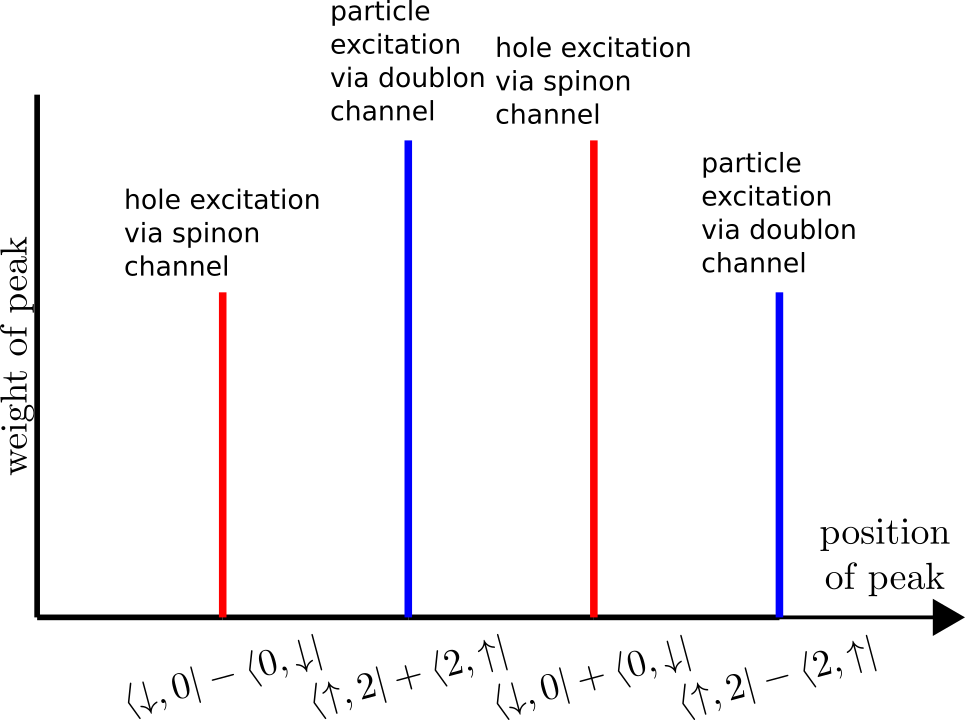
\includegraphics[width=0.9\textwidth]{dimer-peaks.png}
	\caption{Position, weight and nature of each of the peaks in the Hubbard dimer site local spectral function}
\end{figure}

\section*{Appendix: Relation between single-particle Greens function and the Greens function operator $(T=0)$}
 The single-particle Greens function is defined as the solution of the equation:
 \begin{equation}\begin{aligned}
	 \left(i\partial_t - H(\vec r)\right)G(\vec r,\vec r^\prime, t) = \delta(\vec r - \vec r^\prime)
 \end{aligned}\end{equation}
 and is given by the expression
 \begin{equation}\begin{aligned}
	 G(\vec r,\vec r^\prime, t) = -i \theta(t) \left< \left\{ c(\vec r, t) c^\dagger(\vec r^\prime, 0)\right\} \right>
 \end{aligned}\end{equation}
 This solution can be written in the Lehmann representation  and at $T=0$ as
 \begin{equation}\begin{aligned}
	 G(\vec r \sigma, \vec r^\prime \sigma, \omega) = \sum_{n}\left[\frac{\bra{GS}c({\vec r,\sigma})\ket{n}\bra{n}c^\dagger(\vec r^\prime,\sigma)\ket{GS}}{\omega + E_{GS} - E_n} + \frac{\bra{GS}c^\dagger(\vec r^\prime,\sigma)\ket{n}\bra{n}c({\vec r,\sigma})\ket{GS}}{\omega + E_n - E_{GS}}\right]
 \end{aligned}\end{equation}
 The sum is over the exact eigenstates of the Hamiltonian. In what follows, we will represent $\vec r,\sigma \equiv \nu$ and $\vec r^\prime,\sigma \equiv \nu^\prime$.
 \begin{equation}\begin{aligned}
	 G(\nu, \nu^\prime, \omega) &= \sum_{n}\left[\frac{\bra{GS}c(\nu)\ket{n}\bra{n}c^\dagger(\nu^\prime)\ket{GS}}{\omega + E_{GS} - E_n} + \frac{\bra{GS}c^\dagger(\nu^\prime)\ket{n}\bra{n}c(\nu)\ket{GS}}{\omega + E_n - E_{GS}}\right]\\
							&= \bra{GS}c(\nu)\frac{1}{\omega + E_{GS} - H}c^\dagger(\nu^\prime)\ket{GS} + \bra{GS}c^\dagger(\nu^\prime)\frac{1}{\omega + H - E_{GS}}c(\nu)\ket{GS}\\
 \end{aligned}\end{equation}
 If we now define a Greens function operator
 \begin{equation}\begin{aligned}
	 \label{inv_G_func}
	 \mathcal{G}(\omega, H) = \frac{1}{\omega - (H - E_\text{GS})}
 \end{aligned}\end{equation}
 we can write the single-particle Greens function as a sum of the matrix elements of this operator:
 \begin{equation}\begin{aligned}
	 \label{G_mat_el}
	 G(\nu, \nu^\prime, \omega) = \bra{\nu} \mathcal{G}(\omega, H) \ket{\nu^\prime} - \bra{\overline{\nu^\prime}} \mathcal{G}(-\omega, H) \ket{\overline\nu} = \mathcal{G}(\omega, H)_{\nu,\nu^\prime} - \mathcal{G}(-\omega, H)_{\overline{\nu^\prime}, \overline\nu}
 \end{aligned}\end{equation}
 where we have defined the states $\ket{\nu} \equiv c^\dagger(\nu)\ket{GS}$ and $\ket{\overline\nu} \equiv c(\nu)\ket{GS}$. The two matrix elements can also be represented in their individual spectral representations:
 \begin{equation}\begin{aligned}
	 \label{G_mat_spec}
 	\mathcal{G}(\omega, H)_{\nu,\nu^\prime} = \sum_{n}\frac{\bra{GS}c(\nu)\ket{n}\bra{n}c^\dagger(\nu^\prime)\ket{GS}}{\omega + E_{GS} - E_n}\\
	\mathcal{G}(\omega, H)_{\overline{\nu^\prime}, \overline\nu} = \sum_{n}\frac{\bra{GS}c^\dagger(\nu^\prime)\ket{n}\bra{n}c(\nu)\ket{GS}}{\omega + E_\text{GS} - E_n}
 \end{aligned}\end{equation}
 
\section{Appendix: Writing single-particle excitations of ground state in terms of $N=3, S^z = \frac{1}{2}$ eigenstates}
The excited state $c^\dagger_{0\uparrow}\ket{\text{GS}}$ can actually be written in terms of the $N=3$, $S^z = + \frac{1}{2}$ eigenstates $\ket{3\pm\uparrow}$ defined in table \ref{hubb_dim_spectrum}.
\begin{equation}\begin{aligned}
	\ket{3\pm \uparrow} = \frac{1}{\sqrt 2}\left(\ket{\uparrow, 2} \pm \ket{2, \uparrow}\right), && H^D \ket{3\pm \uparrow} = \pm t\ket{3\pm \uparrow}
\end{aligned}\end{equation}
In terms of these eigenstates, we can write
\begin{equation}\begin{aligned}
	c^\dagger_{0\uparrow}\ket{\text{GS}} 
	&= c^\dagger_{0\uparrow}\left[a_1 \ket{SS} + a_2 \ket{CT}\right] \\
	&= a_2 \frac{1}{\sqrt 2}\ket{\uparrow,2} - a_1 \frac{1}{\sqrt 2}\ket{2, \uparrow}\\
	&= \left(x + y\right) \frac{1}{\sqrt 2}\ket{\uparrow,2} + \left(x - y\right) \frac{1}{\sqrt 2}\ket{2, \uparrow}\\
	&=x\ket{3+ \uparrow} + y\ket{3- \uparrow}
\end{aligned}\end{equation}
where $x + y \equiv a_2$ and $x-y \equiv -a_1$. Similarly, for the other site excitation, we can write
\begin{equation}\begin{aligned}
	c^\dagger_{1\uparrow}\ket{\text{GS}} 
	&= c^\dagger_{1\uparrow}\left[a_1 \ket{SS} + a_2 \ket{CT}\right] \\
	&= a_2 \frac{1}{\sqrt 2}\ket{2, \uparrow} - a_1 \frac{1}{\sqrt 2}\ket{\uparrow, 2}\\
	&=  \left(x + y\right) \frac{1}{\sqrt 2}\ket{2, \uparrow} + \left(x - y\right) \frac{1}{\sqrt 2}\ket{\uparrow, 2}\\
	&=x\ket{3+ \uparrow} - y\ket{3- \uparrow}
\end{aligned}\end{equation}
Solving for $x$ and $y$ gives
\begin{equation}\begin{aligned}
	x = \frac{a_2 - a_1}{2}, && y = \frac{a_2 + a_1}{2}
\end{aligned}\end{equation}
Similarly, we can also write the single-hole excitation $c_{0 \uparrow}\ket{GS}$ in terms of the $N=1, S^z = -\frac{1}{2}$ eigenstates, $\ket{1\pm \downarrow}$:
\begin{equation}\begin{aligned}
	\ket{1\pm \downarrow} = \frac{1}{\sqrt 2}\left(\ket{\downarrow, 0} \pm \ket{0, \downarrow}\right), && H^D \ket{1\pm \downarrow} = \mp t\ket{1\pm \downarrow}
\end{aligned}\end{equation}
\begin{equation}\begin{aligned}
	c_{0 \uparrow}\ket{GS} = a_1 \frac{1}{\sqrt 2}\ket{0, \downarrow} + a_2 \frac{1}{\sqrt 2}\ket{\downarrow, 0} = y\ket{1+ \downarrow} + x\ket{1- \downarrow}\\
	c_{1 \uparrow}\ket{GS} = a_1 \frac{1}{\sqrt 2}\ket{\downarrow, 0} + a_2 \frac{1}{\sqrt 2}\ket{0, \downarrow} = y\ket{1+ \downarrow} - x\ket{1- \downarrow}\\
\end{aligned}\end{equation}



\section{Appendix: Matrix elements of $G^{-1}$ between single-particle momentum excitations, for the Hubbard dimer}
\begin{equation}\begin{aligned}
	G^{-1} \equiv \omega + E_\text{GS} - H_D
\end{aligned}\end{equation}
The particle excitation momentum space kets are $\ket{k_0} = \frac{1}{\sqrt 2}\left(\ket{0} + \ket{1}\right) ,\ket{k_\pi} = \frac{1}{\sqrt 2}\left(\ket{0} - \ket{1}\right)$. Therefore,
\begin{equation}\begin{aligned}
	\left(G^{-1}\right)_{k_0 k_0} &= \frac{1}{2}\left(\bra{0} + \bra{1}\right)\left(\omega + E_\text{GS} - H_D\right)\left(\ket{0} + \ket{1}\right)\\
				      &= \frac{1}{2}\left(2x\bra{+}\right)\left(\omega + E_\text{GS} - H_D\right)\left(2x\ket{+}\right)\\
				      &= 2x^2\left(\omega + E_\text{GS} - t\right)\\
\end{aligned}\end{equation}
At the final step, we used $\braket{+,+} = 1$ and $\braket{+|H_D|+} = t$.
\bibliographystyle{unsrt}
\bibliography{notes}
\end{document}
